% Documents setup
\documentclass[french,11pt]{book}

% fix for pandoc 1.14
\providecommand{\tightlist}{%
  \setlength{\itemsep}{0pt}\setlength{\parskip}{0pt}}

\usepackage{tabu} % https://tex.stackexchange.com/questions/50332/vertical-spacing-of-a-table-cell

% Location of the csas-style repository: adjust path as needed
\newcommand{\locRepo}{csas-style}

% Use the style file in the csas-style repository (res-doc.sty)
\usepackage{\locRepo/res-doc-french}

% header-includes from R markdown entry


% Headers and footers
\lhead{}
% \lhead{}
\rhead{}
% \rfoot{DRAFT - DO NOT CITE}

%%%% Commands for title page etc %%%%%

% Publication year
\newcommand{\rdYear}{2021}

% Publication month
\newcommand{\rdMonth}{}

% Report number
\newcommand{\rdNumber}{8}

% Region
\newcommand{\rdRegion}{Pacific Region}

% Title
\newcommand{\rdTitle}{Évaluation des stratégies de rétablissement possibles pour le sébaste aux yeux jaunes (\emph{Sebastes ruberrimus}) des eaux intérieures de la Colombie-Britannique}

\newcommand{\rdISBN}{Fs70-5/2021-008F-PDF}
\newcommand{\rdCatNo}{978-0-660-38699-7}

% Author names separated by commas and ', and' for the last author in the format 'M.H. Grinnell' (use \textsuperscript{n} for addresses)
\newcommand{\rdAuth}{Dana R. Haggarty\textsuperscript{1}, Quang C. Huynh\textsuperscript{2}, Robyn E. Forrest\textsuperscript{1}, Sean C. Anderson\textsuperscript{1}, Midoli J. Bresch\textsuperscript{1}, Elise A. Keppel\textsuperscript{1}}

% Author names reversed separated by commas in the format 'Grinnell, M.H.'
\newcommand{\rdAuthRev}{Haggarty, D.R., C.R. Huynh, R.E. Forrest, S.C. Anderson, M.J. Bresch, et E.A. Keppel}

% Author addresses (use \textsuperscript{n})
\newcommand{\rdAuthAddy}{\textsuperscript{1}Station biologique du Pacifique\\
Pêches et Océans Canada, 3190, chemin Hammond Bay\\
Nanaimo (Colombie-Britannique) V9T 6N7, Canada\\

\textsuperscript{2}Institut pour les océans et la pêche\\
LRAE de l'Université de la Colombie- Britannique, 2202, Main Mall\\
Vancouver (Colombie-Britannique) V6T 1Z4, Canada\\}

\newcommand{\citationOtherLanguage}{Haggarty, D.R., Huynh, Q.C., Forrest, R.E., Anderson, S.C., Bresch, M.J., Keppel, E.A. 2021. Evaluation of potential rebuilding strategies for Inside Yelloweye Rockfish (\emph{Sebastes ruberrimus}) in British Columbia. DFO Can. Sci. Advis. Sec. Res. Doc. 2021/008. vi + 141 p.}

% Name of file with abstract and resume (see \abstract and \frenchabstract for requirements)
\newcommand{\rdAbstract}{\abstract{En vertu des politiques et de la législation canadiennes, il faut Eétablir un plan de rétablissement pour les stocks de poissons qui ont été évalués comme étant inférieurs au point de référence limite (PRL) afin de les ramener au-delà du PRL. Les plans de rétablissement doivent être fondés sur des objectifs caractérisés par 1) une cible, 2) un délai souhaité pour atteindre la cible et 3) une probabilité acceptable d'atteindre la cible. Les plans de rétablissement doivent également comprendre des mesures de gestion ou des procédures de gestion, des jalons cibles et être évalués régulièrement. \vspace{1.5mm} \break Le stock de sébaste aux yeux jaunes (\emph{Sebastes ruberrimus}) des eaux intérieures est un stock sur lequel on dispose de données limitées, présent dans la zone de gestion du poisson de fond 4B (détroit de la Reine-Charlotte, détroit de Georgie et détroit de Juan de Fuca) en Colombie-Britannique. Il a été évalué comme étant inférieur au PLR en 2010, ce qui a donné lieu à la publication d'un plan de rétablissement. Il est également inscrit en vertu de la \emph{Loi sur les espèces en péril} comme espèce préoccupante. L'actuelle procédure de gestion pour assurer le rétablissement est un total autorisé des captures (TAC) annuel fixe de 15 tonnes métriques, qui n'a pas été réévalué depuis la dernière évaluation. \vspace{1.5mm} \break Ce projet vise à fournir un avis scientifique à l'appui de la réévaluation du plan de rétablissement du sébaste aux yeux jaunes des eaux intérieures. Nous appliquons un nouveau cadre d'évaluation de la stratégie de gestion (le Cadre des procédures de gestion), récemment élaboré pour le poisson de fond de la Colombie-Britannique, afin d'évaluer le rendement des autres procédures de gestion à données limitées pour ce qui est de l'atteinte des objectifs de rétablissement. Le Cadre des procédures de gestion suit six étapes de pratiques exemplaires pour évaluer la stratégie de gestion~: 1) la définition du contexte décisionnel; 2) l'établissement des objectifs et des paramètres de rendement; 3) la précision des modèles opérationnels pour représenter le système sous-jacent et calculer les paramètres de rendement; 4) la sélection des procédures de gestion possibles; 5) la réalisation de simulations en boucle fermée afin d'évaluer le rendement des procédures de gestion; 6) la présentation des résultats pour faciliter l'évaluation des compromis. \vspace{1.5mm} \break Nous avons appliqué ce cadre pour évaluer le rendement de 34 procédures de gestion à données limitées pour ce qui est de l'atteinte de l'objectif principal, qui est de ramener le stock au-dessus du PRL sur 1,5 génération avec au moins une probabilité de réussite de 95 \% {[}19 fois sur 20{]}. Nous avons également évalué le rendement des procédures de gestion en ce qui concerne deux autres paramètres de conservation, quatre objectifs de prises moyennes et un objectif de variabilité des prises. Pour tenir compte de l'incertitude liée à la dynamique de la population sous-jacente et aux sources de données, nous avons élaboré six scénarios de modèles opérationnels de rechange, qui différaient de par les hypothèses précises du modèle et des données. Ces scénarios de modèles opérationnels ont été divisés en un « ensemble de référence » (quatre modèles opérationnels) et un « ensemble de robustesse » (deux modèles opérationnels). Nous avons conditionné tous les modèles opérationnels aux données sur les prises observées, aux indices de l'abondance et aux données accessibles sur la composition selon l'âge. Nous avons utilisé la simulation en boucle fermée pour évaluer le rendement des procédures de gestion et nous avons éliminé celles qui ne satisfaisaient pas à un ensemble de critères de base, ce qui a laissé cinq procédures de gestion possibles~: des procédures de gestion à prises constantes annuelles de 10 ou 15 tonnes et trois procédures de gestion qui ajustent le TAC en fonction de la pente relative de l'indice de l'abondance dans le relevé à la palangre sur fond dur dans les eaux intérieures. \vspace{1.5mm} \break Les cinq procédures de gestion finales atteignaient l'objectif principal avec une probabilité supérieure à 0,98 (49 fois sur 50), dans les scénarios des quatre modèles opérationnels de l'ensemble de référence, surtout qu'aucun des modèles opérationnels de l'ensemble de référence n'a estimé que le stock serait inférieur au PRL en 2020. Dans les scénarios des deux modèles opérationnels de l'ensemble de robustesse, le scénario qui simulait une plus grande variabilité dans le futur relevé à la palangre sur fond dur a donné des résultats semblables à ceux des scénarios de l'ensemble de référence. Cependant, dans le scénario qui supposait un taux de mortalité naturelle plus faible pour le stock (« M faible »), toutes les procédures de gestion avaient des probabilités plus basses d'atteindre l'objectif principal, la probabilité la plus faible étant atteinte par la procédure de gestion actuelle (prises constantes de 15 tonnes). \vspace{1.5mm} \break Nous présentons un certain nombre de visualisations pour illustrer les compromis entre les objectifs de conservation et de prises pour les différentes procédures de gestion dans d'autres scénarios de modèles opérationnels. Ces visualisations présentent les compromis sous forme de tableaux et de graphiques, destinés à faciliter le processus de sélection de la procédure de gestion finale. Étant donné que toutes les procédures de gestion ont atteint l'objectif principal dans les scénarios de l'ensemble de référence, il n'y avait pas de compromis important entre les objectifs de conservation et les objectifs de prises. Parmi les deux scénarios de l'ensemble de robustesse, les compromis étaient les plus évidents dans le scénario de M faible, où la probabilité d'atteindre l'objectif principal diminuait à mesure que la probabilité de prises moyennes à court terme de 10 tonnes augmentait. \vspace{1.5mm} \break Nous discutons des incertitudes majeures, y compris l'incertitude entourant la mortalité naturelle, la sélectivité et les prises historiques, en notant que nous avons tenté d'en tenir compte en évaluant le rendement des procédures de gestion dans plusieurs modèles opérationnels. Nous soulignons les problèmes concernant les estimations de l'état actuel du stock de sébaste aux yeux jaunes des eaux intérieures et le rôle des points de référence dans le Cadre des procédures de gestion. Nous formulons des recommandations sur la fréquence des évaluations et suggérons des déclencheurs pour la réévaluation. Nous évaluons également le rendement des procédures de gestion en ce qui concerne le respect de deux autres critères d'évaluation pour le Comité sur la situation des espèces en péril au Canada.}}

%%%% End of title page commands %%%%%

% \pdfcompresslevel=5 % faster PNGs

\setcounter{section}{0}

\bibliographystyle{csas-style/res-doc}

\usepackage{amsmath}
\usepackage{bm}

% commands and environments needed by pandoc snippets
% extracted from the output of `pandoc -s`
%% Make R markdown code chunks work
\usepackage{array}
\usepackage{amssymb,amsmath}
\usepackage{color}
\usepackage{fancyvrb}
% From default template:
\newcommand{\VerbBar}{|}
\newcommand{\VERB}{\Verb[commandchars=\\\{\}]}
\DefineVerbatimEnvironment{Highlighting}{Verbatim}{commandchars=\\\{\}}
% Add ',fontsize=\small' for more characters per line
\usepackage{framed}
\definecolor{shadecolor}{RGB}{248,248,248}
\newenvironment{Shaded}{\begin{snugshade}}{\end{snugshade}}
\newcommand{\AlertTok}[1]{\textcolor[rgb]{0.94,0.16,0.16}{#1}}
\newcommand{\AnnotationTok}[1]{\textcolor[rgb]{0.56,0.35,0.01}{\textbf{\textit{#1}}}}
\newcommand{\AttributeTok}[1]{\textcolor[rgb]{0.77,0.63,0.00}{#1}}
\newcommand{\BaseNTok}[1]{\textcolor[rgb]{0.00,0.00,0.81}{#1}}
\newcommand{\BuiltInTok}[1]{#1}
\newcommand{\CharTok}[1]{\textcolor[rgb]{0.31,0.60,0.02}{#1}}
\newcommand{\CommentTok}[1]{\textcolor[rgb]{0.56,0.35,0.01}{\textit{#1}}}
\newcommand{\CommentVarTok}[1]{\textcolor[rgb]{0.56,0.35,0.01}{\textbf{\textit{#1}}}}
\newcommand{\ConstantTok}[1]{\textcolor[rgb]{0.00,0.00,0.00}{#1}}
\newcommand{\ControlFlowTok}[1]{\textcolor[rgb]{0.13,0.29,0.53}{\textbf{#1}}}
\newcommand{\DataTypeTok}[1]{\textcolor[rgb]{0.13,0.29,0.53}{#1}}
\newcommand{\DecValTok}[1]{\textcolor[rgb]{0.00,0.00,0.81}{#1}}
\newcommand{\DocumentationTok}[1]{\textcolor[rgb]{0.56,0.35,0.01}{\textbf{\textit{#1}}}}
\newcommand{\ErrorTok}[1]{\textcolor[rgb]{0.64,0.00,0.00}{\textbf{#1}}}
\newcommand{\ExtensionTok}[1]{#1}
\newcommand{\FloatTok}[1]{\textcolor[rgb]{0.00,0.00,0.81}{#1}}
\newcommand{\FunctionTok}[1]{\textcolor[rgb]{0.00,0.00,0.00}{#1}}
\newcommand{\ImportTok}[1]{#1}
\newcommand{\InformationTok}[1]{\textcolor[rgb]{0.56,0.35,0.01}{\textbf{\textit{#1}}}}
\newcommand{\KeywordTok}[1]{\textcolor[rgb]{0.13,0.29,0.53}{\textbf{#1}}}
\newcommand{\NormalTok}[1]{#1}
\newcommand{\OperatorTok}[1]{\textcolor[rgb]{0.81,0.36,0.00}{\textbf{#1}}}
\newcommand{\OtherTok}[1]{\textcolor[rgb]{0.56,0.35,0.01}{#1}}
\newcommand{\PreprocessorTok}[1]{\textcolor[rgb]{0.56,0.35,0.01}{\textit{#1}}}
\newcommand{\RegionMarkerTok}[1]{#1}
\newcommand{\SpecialCharTok}[1]{\textcolor[rgb]{0.00,0.00,0.00}{#1}}
\newcommand{\SpecialStringTok}[1]{\textcolor[rgb]{0.31,0.60,0.02}{#1}}
\newcommand{\StringTok}[1]{\textcolor[rgb]{0.31,0.60,0.02}{#1}}
\newcommand{\VariableTok}[1]{\textcolor[rgb]{0.00,0.00,0.00}{#1}}
\newcommand{\VerbatimStringTok}[1]{\textcolor[rgb]{0.31,0.60,0.02}{#1}}
\newcommand{\WarningTok}[1]{\textcolor[rgb]{0.56,0.35,0.01}{\textbf{\textit{#1}}}}

\newcommand{\lt}{\ensuremath <}
\newcommand{\gt}{\ensuremath >}

%Defines cslreferences environment
%Required by pandoc 2.8
%Copied from https://github.com/rstudio/rmarkdown/issues/1649

\DeclareGraphicsExtensions{.png,.pdf}
\begin{document}
\renewcommand{\tablename}{Tableau}
\frontmatter

\clearpage

\hypertarget{sec:introduction}{%
\section{INTRODUCTION}\label{sec:introduction}}

Ce projet vise à fournir un avis scientifique à l'appui de la révision du plan de rétablissement du stock de sébaste aux yeux jaunes (\emph{Sebastes ruberrimus}) des eaux intérieures (DFO \protect\hyperlink{ref-ifmp2018}{2018}), conformément aux directives stratégiques nationales (DFO \protect\hyperlink{ref-dfo2009}{2009}, \protect\hyperlink{ref-dfo2013}{2013}). Il applique un cadre de simulation en boucle fermée (Anderson et al. \protect\hyperlink{ref-anderson2020gfmp}{2020}\protect\hyperlink{ref-anderson2020gfmp}{a}) pour évaluer le rendement des procédures de gestion de rechange en ce qui concerne les objectifs de rétablissement du stock de sébaste aux yeux jaunes des eaux intérieures.

\hypertarget{sec:introduction-motivation}{%
\subsection{MOTIVATION~: OBLIGATIONS STRATÉGIQUES ET LÉGISLATIVES}\label{sec:introduction-motivation}}

Le Cadre pour la pêche durable du Canada jette les bases de l'approche de précaution en matière de gestion des pêches au Canada (DFO \protect\hyperlink{ref-dfo2006}{2006}, \protect\hyperlink{ref-dfo2009}{2009}). Le Cadre de l'approche de précaution (DFO \protect\hyperlink{ref-dfo2009}{2009}) repose sur la définition des points de référence biologiques qui définissent les cibles de la biomasse ainsi que les seuils de biomasse faible à éviter avec une probabilité élevée. L'approche exige que la mortalité par pêche soit ajustée par rapport à deux niveaux de l'état des stocks~: un point de référence supérieur du stock (RSS) et un point de référence limite (PRL) (figure~\ref{fig:pa-illustration}). Le PRL et le RSS délimitent trois zones d'état des stocks (« critique », « de prudence » et « saine »). Il faut établir un plan de rétablissement pour les stocks de poissons canadiens qui ont été évalués comme étant inférieurs au PRL, c.-à-d.~dans la zone critique (DFO \protect\hyperlink{ref-dfo2009}{2009}), afin de les ramener au-dessus du PRL (DFO \protect\hyperlink{ref-dfo2013}{2013}).


\begin{figure}[htb]

{\centering \pdftooltip{\includegraphics[width=3.8in]{C:/GitHub/yelloweye-inside/figs-french/pa-framework}}{Figure \ref{fig:pa-illustration}} 

}

\caption{Illustration du Cadre de l'approche de précaution du MPO. D'après DFO (\protect\hyperlink{ref-dfo2009}{2009}).}\label{fig:pa-illustration}
\end{figure}
En juin 2019, d'importantes modifications apportées à la \emph{Loi sur les pêches} du Canada ont légiféré de nombreux éléments clés du Cadre pour la pêche durable, qui sont enchâssés dans les dispositions sur les stocks de poissons (\href{https://laws-lois.justice.gc.ca/fra/lois/f-14/page-3.html\#h-1175547}{article 6 de la \emph{Loi sur les pêches}}. Les dispositions relatives aux stocks de poissons exigent que les principaux stocks soient gérés à des niveaux durables, en particulier à des niveaux de biomasse supérieurs au PRL. De plus, le paragraphe 6.2(1) stipule que si un grand stock de poissons a diminué en deçà de son PRL, un plan de rétablissement doit être établi pour reconstituer le stock au-dessus du PRL. Les grands stocks de poissons seront désignés en vertu d'un règlement, le premier lot de stocks devant l'être à l'automne 2020.

En vertu des directives sur l'élaboration de plans de rétablissement au Canada (DFO \protect\hyperlink{ref-dfo2013}{2013}), les plans de rétablissement doivent être fondés sur des objectifs caractérisés par~:
\begin{enumerate}
\def\labelenumi{\arabic{enumi}.}

\item
  une cible;
\item
  un délai souhaité pour atteindre la cible;
\item
  une probabilité acceptable convenue d'atteindre la cible.
\end{enumerate}
Les plans de rétablissement doivent également comprendre des mesures de gestion planifiées (les procédures de gestion), des jalons cibles et leur rendement doit faire l'objet d'examens réguliers (tous les trois ans), en plus de la surveillance et de l'évaluation annuelles. Les directives actuelles indiquent que le délai de rétablissement doit être de 1,5 à 2 fois la durée de génération de l'espèce (DFO \protect\hyperlink{ref-dfo2013}{2013}), la durée de génération étant le nombre moyen d'années entre la naissance d'un individu et la naissance de sa progéniture.

\hypertarget{sec:introduction-background}{%
\subsection{CONTEXTE}\label{sec:introduction-background}}

Le sébaste aux yeux jaunes des eaux intérieures est présent dans la zone de gestion 4B du poisson de fond en Colombie-Britannique (Figure~\ref{fig:map-4B}). Il devrait être désigné comme grand stock de poissons à l'automne 2020, date à laquelle sa gestion sera légiférée en vertu des dispositions sur les stocks de poissons. Le stock a été évalué comme étant inférieur au PLR en 2010 (Yamanaka et al. \protect\hyperlink{ref-yamanaka2011}{2011}; DFO \protect\hyperlink{ref-dfo2012}{2012}). De ce fait, un plan de rétablissement a été élaboré et publié à l'annexe 9 du Plan de gestion intégrée des pêches de la région du Pacifique pour le poisson de fond (DFO \protect\hyperlink{ref-ifmp2018}{2018}). Le stock de sébaste aux yeux jaunes des eaux intérieures est également inscrit en vertu de la \emph{Loi sur les espèces en péril} (LEP) comme espèce préoccupante (COSEWIC \protect\hyperlink{ref-cosewic2008}{2008}) et il est prévu que le Comité sur la situation des espèces en péril au Canada (COSEPAC) le réévaluera en 2020. Les résultats de ce projet pourraient guider la réévaluation du COSEPAC et, éventuellement, une évaluation du potentiel de rétablissement en vertu de la LEP, s'il y a lieu (voir l'annexe~\ref{app:cosewic}).


\begin{figure}[htb]

{\centering \pdftooltip{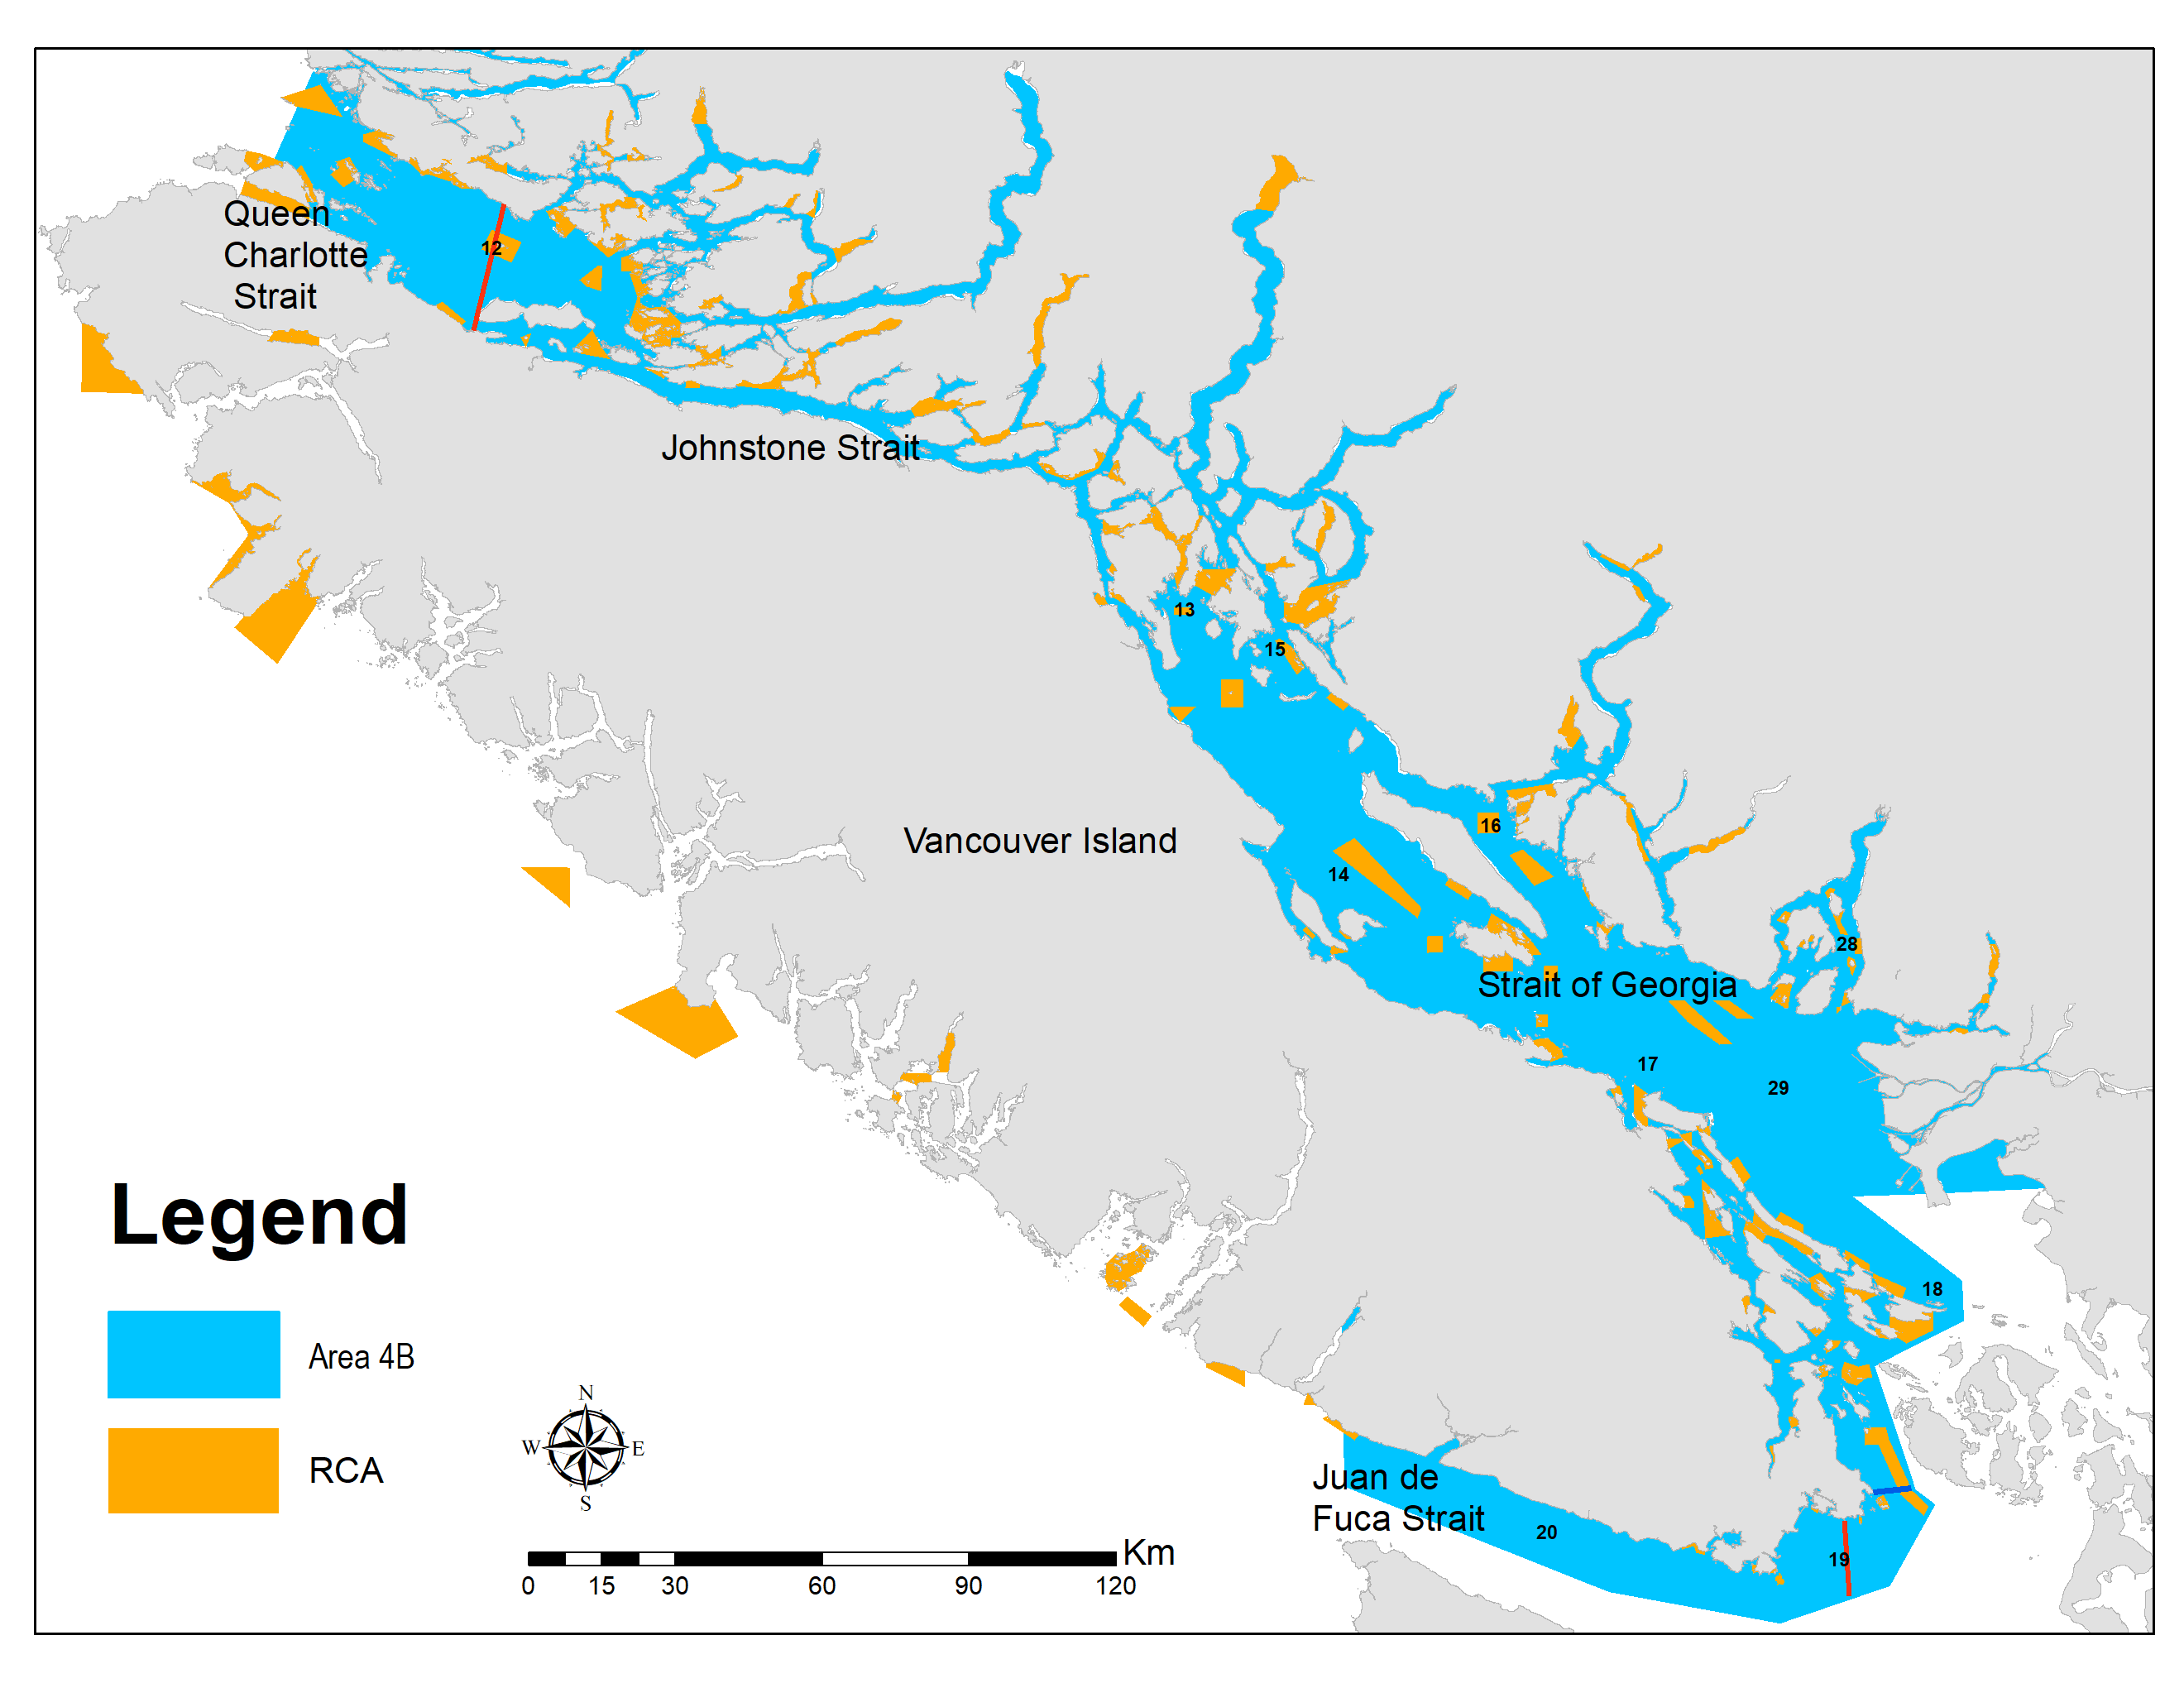
\includegraphics[width=5in]{C:/GitHub/yelloweye-inside/figs-french/InsideYE_Map_new}}{Figure \ref{fig:map-4B}} 

}

\caption{Carte de la zone de gestion 4B du poisson de fond montrant les aires de conservation du sébaste (ACS) et les limites séparant l'unité désignable (UD) du sébaste aux yeux jaunes des eaux intérieures de l'UD du sébaste aux yeux jaunes des eaux extérieures. Les lignes rouges indiquent une proposition d'ajustement de l'aire de répartition de l'UD des eaux intérieures, fondée sur des preuves génétiques récentes (Siegle \protect\hyperlink{ref-siegle2011}{2011}; Siegle et al. \protect\hyperlink{ref-siegle2013}{2013}; Andrews et al. \protect\hyperlink{ref-andrews2018}{2018}).}\label{fig:map-4B}
\end{figure}
L'objectif du plan de rétablissement actuel est de « reconstituer le stock au-dessus du PRL sur 80 ans avec une probabilité de réussite de 56 \% ». Le jalon cible est de « dégager des tendances positives au cours de chaque période de 10 ans ». La procédure de gestion actuelle du sébaste aux yeux jaunes des eaux intérieures vise à maintenir les prises annuelles totales (commerciales, récréatives, alimentaires, sociales et rituelles des Premières Nations et de relevé) à moins de 15 tonnes (voir l'annexe 9 du document DFO (\protect\hyperlink{ref-ifmp2018}{2018}) pour plus de renseignements).

D'après les directives, les plans de rétablissement au Canada doivent présenter une forte probabilité de rétablissement des stocks de poissons hors de la zone critique dans le délai prescrit (DFO \protect\hyperlink{ref-dfo2013}{2013}). Ce projet vise notamment à répondre à une préoccupation exprimée par les gestionnaires des pêches, à savoir que la probabilité de réussite de 56 \% énoncée dans le plan de rétablissement actuel (DFO \protect\hyperlink{ref-ifmp2018}{2018}) ne correspond pas à la définition d'une probabilité élevée.

Le document d'orientation indique également certaines mesures de gestion recommandées, comme le maintien des prélèvements par toutes les sources au niveau le plus bas possible, l'élaboration d'une règle de contrôle des prises et l'application de l'évaluation de la stratégie de gestion pour évaluer, par simulation, le rendement d'autres mesures de gestion pour atteindre les objectifs de rétablissement du stock (DFO \protect\hyperlink{ref-dfo2013}{2013}). Le plan de rétablissement actuel met en œuvre un total autorisé des captures annuel fixe de 15 tonnes (DFO \protect\hyperlink{ref-ifmp2018}{2018}), qui n'a pas été mis à l'essai par simulation.

Le sébaste aux yeux jaunes est une espèce qui vit longtemps (jusqu'à 121 ans en Colombie-Britannique, Keppel et Olsen \protect\hyperlink{ref-keppel2019}{2019}), dans des habitats démersaux rocheux répartis de manière irrégulière et discontinue sur la côte intérieure de la Colombie-Britannique (Yamanaka et al. \protect\hyperlink{ref-yamanaka2011}{2011}). Ces caractéristiques du cycle biologique rendent l'espèce vulnérable à la surexploitation par la pêche. Le stock des eaux intérieures est considéré comme étant à données limitées, car peu de données sont accessibles sur la composition selon l'âge, on manque de données biologiques sur les pêches commerciales, récréatives et des Premières Nations, et une incertitude entoure l'ampleur des prises historiques.

\hypertarget{sec:introduction-mse}{%
\subsection{ÉVALUATION DE LA STRATÉGIE DE GESTION}\label{sec:introduction-mse}}

À l'échelle mondiale, la fourniture d'avis scientifiques pour la gestion des pêches a évolué vers des approches axées sur l'évaluation de la stratégie de gestion (ou axées sur la gestion) (p.~ex., Butterworth et Punt \protect\hyperlink{ref-butterworth1999}{1999}; Rademeyer et al. \protect\hyperlink{ref-rademeyer2007}{2007}; Berkson et Thorson \protect\hyperlink{ref-berkson2015}{2015}; Geromont et Butterworth \protect\hyperlink{ref-geromont2015}{2015}; Carruthers et al. \protect\hyperlink{ref-carruthers2016}{2016}; Punt et al. \protect\hyperlink{ref-punt2016}{2016}). L'évaluation de la stratégie de gestion se concentre sur la détermination des procédures de gestion qui donnent les meilleurs résultats en ce qui concerne l'atteinte des objectifs convenus en matière de politique et de pêche, lorsqu'ils sont mis en œuvre dans un environnement de simulation en « boucle fermée » (figure~\ref{fig:mse-chart-basic}). Dans les pêches à production contrôlée, comme la pêche du poisson de fond en Colombie-Britannique, où les quotas sont gérés, les procédures de gestion décrivent les mesures de gestion pour l'établissement des limites des prises. Les données exigées dans les procédures de gestion peuvent varier considérablement, allant d'approches très riches en données, y compris les évaluations statistiques des prises selon l'âge avec des règles de contrôle des prises, à des règles de données simples (approches « limitées en données »), qui ne reposent que sur les données sur les prises et un indice de l'abondance (p.~ex., Geromont et Butterworth \protect\hyperlink{ref-geromont2015}{2015}; Carruthers et al. \protect\hyperlink{ref-carruthers2016}{2016}).

La simulation en boucle fermée diffère des approches d'évaluation classique des stocks parce qu'elle simule la rétroaction entre la mise en œuvre des procédures de gestion et le système sous-jacent (le stock de poisson et son environnement), décrite par un ou plusieurs modèles opérationnels. L'approche de la simulation en boucle fermée tient compte de l'effet des procédures de gestion sur le système, ainsi que des données futures recueillies dans le système et de leur utilisation chez les procédures de gestion (Punt et al. \protect\hyperlink{ref-punt2016}{2016}; Carruthers et Hordyk \protect\hyperlink{ref-carruthers2018}{2018}\protect\hyperlink{ref-carruthers2018}{a}; Anderson et al. \protect\hyperlink{ref-anderson2020gfmp}{2020}\protect\hyperlink{ref-anderson2020gfmp}{a}).


\begin{figure}[htb]

{\centering \pdftooltip{\includegraphics[width=6.3in]{C:/GitHub/yelloweye-inside/figs-french/mse-chart-simple2}}{Figure \ref{fig:mse-chart-basic}} 

}

\caption{Illustration du processus de simulation en boucle fermée des pêches d'après Anderson et al. (\protect\hyperlink{ref-anderson2020gfmp}{2020}\protect\hyperlink{ref-anderson2020gfmp}{a}), selon Punt et al. (\protect\hyperlink{ref-punt2016}{2016}). La procédure de gestion peut être fondée sur une règle de données simple (p.~ex., réduire les prises autorisées de x \% si l'indice du relevé diminue de y \%) ou peut être un modèle d'estimation combiné à une règle de contrôle des prises.}\label{fig:mse-chart-basic}
\end{figure}
\hypertarget{sec:introduction-approach}{%
\subsection{APPROCHE}\label{sec:introduction-approach}}

En raison des données limitées sur le stock de sébaste aux yeux jaunes des eaux intérieures, il est difficile d'évaluer le rendement prévu des mesures de gestion nécessaires pour rendre le stock conforme aux dispositions sur les stocks de poissons, c.-à-d.~pour le faire sortir de la zone critique dans le délai convenu et avec la probabilité convenue. La simulation-mise à l'essai en boucle fermée des procédures de gestion à données limitées permet d'évaluer le rendement relatif des procédures de gestion dans un éventail d'incertitudes entourant, par exemple, la biologie sous-jacente des poissons, l'erreur d'observation, l'erreur d'estimation et l'erreur de mise en œuvre (p.~ex., Kell et al. \protect\hyperlink{ref-kell2006}{2006}; Carruthers et al. \protect\hyperlink{ref-carruthers2016}{2016}).

Depuis 2017, une entente de partenariat entre l'Université de la Colombie-Britannique et le MPO (DFO \protect\hyperlink{ref-dfo_dlmtool_2017}{2017}) a facilité l'élaboration de deux progiciels à accès libre pour l'évaluation de la stratégie de gestion, mis en œuvre dans l'environnement de programmation statistique R (R Core Team \protect\hyperlink{ref-r2019}{2019})~: l'outil pour les méthodes à données limitées (DLMtool) (Carruthers et Hordyk \protect\hyperlink{ref-carruthers2018}{2018}\protect\hyperlink{ref-carruthers2018}{a}, \protect\hyperlink{ref-carruthers_hordyk_2018}{2018}\protect\hyperlink{ref-carruthers_hordyk_2018}{b}) et l'outil pour l'évaluation de la stratégie de gestion (MSEtool) (Huynh et al. \protect\hyperlink{ref-huynh_msetool_2019}{2019}). Après plusieurs années de développement, ces progiciels sont parmi les logiciels les plus rapides, les plus souples et les plus extensibles pour évaluer les stratégies de gestion des pêches. Ils peuvent être appliqués à des stocks pauvres ou riches en données, permettant d'évaluer rapidement plusieurs procédures de gestion en fonction d'objectifs de conservation et de pêche personnalisables, et d'évaluer les principaux compromis.

\hypertarget{sec:introduction-mp-framework}{%
\subsubsection{Cadre des procédures de gestion du poisson de fond en Colombie-Britannique}\label{sec:introduction-mp-framework}}

Le Cadre des procédures de gestion pour le poisson de fond en Colombie-Britannique (Anderson et al. \protect\hyperlink{ref-anderson2020gfmp}{2020}\protect\hyperlink{ref-anderson2020gfmp}{a}) a été élaboré parallèlement au présent document pour évaluer le rendement d'un large éventail de procédures de gestion pour les espèces de poisson de fond à données limitées. Le Cadre des procédures de gestion fait largement appel aux fonctions de DLMtool et de MSEtool, avec l'appui d'un progiciel R gfdlm (Anderson et al. \protect\hyperlink{ref-gfdlm}{2020}\protect\hyperlink{ref-gfdlm}{c}) rédigé par les auteurs de Anderson et al. (\protect\hyperlink{ref-anderson2020gfmp}{2020}\protect\hyperlink{ref-anderson2020gfmp}{a}), qui contient un ensemble d'outils de soutien logiciel et des visualisations personnalisées.

Nous suivons le Cadre des procédures de gestion pour sélectionner les procédures de gestion afin d'établir des limites des prises pour les stocks de poissons de fond à données limitées (Anderson et al. \protect\hyperlink{ref-anderson2020gfmp}{2020}\protect\hyperlink{ref-anderson2020gfmp}{a}). Notre évaluation du plan de rétablissement du sébaste aux yeux jaunes des eaux intérieures constitue la première application du Cadre des procédures de gestion pour produire un avis scientifique à l'appui des décisions sur les prises. Le cadre suit six étapes de pratiques exemplaires décrites ci-après et plus en détail dans Anderson et al. (\protect\hyperlink{ref-anderson2020gfmp}{2020}\protect\hyperlink{ref-anderson2020gfmp}{a}).

Les étapes des pratiques exemplaires sont fondées sur un examen effectué par Punt et al. (\protect\hyperlink{ref-punt2016}{2016}), qui a cerné cinq étapes clés du processus d'évaluation de la stratégie de gestion (étapes 2 à 6 ci-après). Une première étape supplémentaire du Cadre des procédures de gestion, qui définit le contexte décisionnel, a été définie par Gregory et al. (\protect\hyperlink{ref-gregory2012}{2012}) et Cox et Benson (\protect\hyperlink{ref-cox2016}{2016}). En grande partie, le logiciel DLMtool a été conçu pour permettre aux praticiens de suivre ces étapes (figure~\ref{fig:mse-chart}; Carruthers et Hordyk \protect\hyperlink{ref-carruthers2018}{2018}\protect\hyperlink{ref-carruthers2018}{a}).



Les six étapes sont les suivantes~:

Étape 1~: Définition du contexte décisionnel.

Étape 2~: Choix des objectifs et des paramètres de rendement.

Étape 3~: Choix des incertitudes/spécification des modèles opérationnels.

Étape 4~: Détermination des procédures de gestion possibles.

Étape 5~: Simulation de l'application des procédures de gestion.

Étape 6~: Présentation des résultats et choix de la procédure de gestion.

\clearpage
\begin{figure}[htb]

{\centering \pdftooltip{\includegraphics[width=\textwidth]{C:/GitHub/yelloweye-inside/figs-french/mse-chart}}{Figure \ref{fig:mse-chart}} 

}

\caption{Les étapes du processus d'évaluation de la stratégie de gestion selon Punt et al. (\protect\hyperlink{ref-punt2016}{2016}), tel que mis en œuvre dans DLMtool. Copié de Anderson et al. (\protect\hyperlink{ref-anderson2020gfmp}{2020}\protect\hyperlink{ref-anderson2020gfmp}{a}) et adapté de Carruthers et Hordyk (\protect\hyperlink{ref-carruthers2018}{2018}\protect\hyperlink{ref-carruthers2018}{a}). Cette figure complète la figure~\ref{fig:mse-chart-basic}.}\label{fig:mse-chart}
\end{figure}
Après la sélection et la mise en œuvre de la procédure de gestion pour l'établissement de la limite des prises (figure~\ref{fig:mse-chart}; par exemple, application de l'algorithme de la procédure de gestion sélectionnée à l'indice du relevé observé), la dernière étape nécessaire consiste à surveiller et à évaluer périodiquement le rendement de la procédure de gestion (DFO \protect\hyperlink{ref-dfo2013}{2013}; Dowling et al. \protect\hyperlink{ref-dowling2015a}{2015}; Carruthers et Hordyk \protect\hyperlink{ref-carruthers2018}{2018}\protect\hyperlink{ref-carruthers2018}{a}). Cela peut se faire par des moyens informels, comme à l'aide de la rétroaction des pêcheurs et des données des relevés (p.~ex., Cox et Kronlund \protect\hyperlink{ref-cox2008a}{2008}), ou au moyen de mesures statistiques plus formelles, où l'on compare les données observées aux prévisions des modèles opérationnels pour vérifier si le système fonctionne comme prévu (Butterworth \protect\hyperlink{ref-butterworth2008}{2008}; Carruthers et Hordyk \protect\hyperlink{ref-carruthers_hordyk_2018}{2018}\protect\hyperlink{ref-carruthers_hordyk_2018}{b}; discussion dans Anderson et al. \protect\hyperlink{ref-anderson2020gfmp}{2020}\protect\hyperlink{ref-anderson2020gfmp}{a}).

Dans les sections suivantes, nous décrivons notre approche pour l'élaboration d'un éventuel plan de rétablissement du sébaste aux yeux jaunes des eaux intérieures, en suivant les six étapes des pratiques exemplaires.

\hypertarget{sec:decision-context}{%
\section{DÉFINIR LE CONTEXTE DÉCISIONNEL}\label{sec:decision-context}}

Les principales questions qui guident la définition du contexte décisionnel de l'évaluation de la stratégie de gestion sont les suivantes~:

\emph{Quelle est la décision exacte à prendre? }Quel est le délai pour prendre la décision? \emph{Quels sont les rôles et responsabilités précis des parties concernées? Les parties sont les Sciences, la Gestion des pêches, les Premières Nations, l'industrie, le milieu universitaire et des organisations non gouvernementales. }Comment la décision finale sera-t-elle prise?

Pour ce plan de rétablissement, il faut décider de la procédure de gestion à utiliser pour déterminer les limites des prises pour la période allant jusqu'au prochain avis disponible sur les prises. Le Comité régional d'examen par les pairs devrait prendre la décision finale sur la procédure de gestion à appliquer pour déterminer les futures limites des prises sur une base consensuelle, après avoir examiné le contenu scientifique de l'avis (y compris la structure et le contenu des modèles opérationnels) et tenu compte du rendement relatif des procédures de gestion et des compromis entre les paramètres de rendement.

\hypertarget{sec:objectives-metrics}{%
\section{SÉLECTION DES OBJECTIFS ET DES PARAMÈTRES DE RENDEMENT}\label{sec:objectives-metrics}}

Il faut établir des objectifs clairs en matière de gestion et de pêche, ainsi que les paramètres de rendement qui permettent de les évaluer. Les objectifs peuvent couvrir un large éventail d'objectifs stratégiques ou législatifs (p.~ex., maintenir le stock au-dessus du PRL), d'objectifs économiques (p.~ex., maintenir des prises moyennes ou réduire la variabilité des prises) et d'objectifs culturels (p.~ex., maintenir l'accès minimal requis au stock ou à des zones de pêche particulières). Dans un scénario de rétablissement, les objectifs de conservation doivent avoir préséance. Cependant, dans un cadre de simulation, il est possible d'examiner des compromis entre la conservation et d'autres objectifs de pêche à court et à long terme, tant que l'objectif principal de conservation est atteint. Les objectifs entièrement quantifiés comprennent un paramètre ou une cible, la probabilité souhaitée de réussite et un délai pour atteindre l'objectif (p.~ex., la probabilité de maintenir le stock au-dessus du PRL est supérieure à 0,95 {[}19 fois sur 20{]} sur 1,5 génération du stock). Les paramètres de rendement sont des mesures quantifiées des objectifs. Dans une simulation en boucle fermée, ils sont calculés dans le modèle opérationnel à chaque étape temporelle des projections.

L'objectif initial du plan de rétablissement était de reconstituer le stock au-dessus du PRL sur 80 ans avec une probabilité de réussite de 56 \%. Un autre jalon cible était d'atteindre des tendances positives de la biomasse dans chaque période de 10 ans. La procédure de gestion convenue pour atteindre ces objectifs était de maintenir le TAC combiné (pêches commerciales, récréatives, ASR, de relevé biologique) à moins de 15 tonnes par année (DFO \protect\hyperlink{ref-ifmp2018}{2018}).

\hypertarget{sec:objectives-metrics-obj}{%
\subsection{OBJECTIFS ET JALONS}\label{sec:objectives-metrics-obj}}

Nous présentons un ensemble d'objectifs améliorés et les paramètres de rendement connexes pour le plan de rétablissement du sébaste aux yeux jaunes des eaux intérieures. Les principaux objectifs provisoires de conservation sont guidés par le Cadre de l'approche de précaution (DFO \protect\hyperlink{ref-dfo2006}{2006}, \protect\hyperlink{ref-dfo2009}{2009}), le document d'orientation du plan de rétablissement (DFO \protect\hyperlink{ref-dfo2013}{2013}) et les précédents régionaux (Cox et al. \protect\hyperlink{ref-cox2019}{2019}, \protect\hyperlink{ref-cox2020}{2020}). D'autres objectifs liés au rendement des pêches et à la variabilité du rendement annuel des pêches sont fondés sur des précédents dans d'autres analyses de la région du Pacifique du MPO (p.~ex., Cox et Kronlund \protect\hyperlink{ref-cox2008a}{2008}; Forrest et al. \protect\hyperlink{ref-forrest2018}{2018}; Cox et al. \protect\hyperlink{ref-cox2019}{2019}, \protect\hyperlink{ref-cox2020}{2020}).

L'objectif de conservation de base proposé est le suivant~:
\begin{enumerate}
\def\labelenumi{\arabic{enumi}.}

\item
  Ramener le stock au-dessus du PRL sur 56 ans (1,5 génération) avec une probabilité de réussite d'au moins 95 \% {[}19 fois sur 20{]}.
\end{enumerate}
Nous avons ajusté le délai de rétablissement initial de 80 ans (DFO \protect\hyperlink{ref-ifmp2018}{2018}) à 56 ans dans la présente analyse, en fonction de la durée de génération estimée pour le sébaste aux yeux jaunes des eaux extérieures (Cox et al. \protect\hyperlink{ref-cox2020}{2020}), en tenant compte de la directive selon laquelle le rétablissement doit être réalisé dans un délai de 1,5 à 2 durées de génération (DFO \protect\hyperlink{ref-dfo2013}{2013}). Pour de plus amples renseignements sur la durée de génération, consulter l'annexe~\ref{app:biological-data}, section~\ref{sec:generation}. Nous avons fait passer la probabilité de réussite souhaitée de 56 \% à 95 \% pour tenir compte de la directive selon laquelle la probabilité de rétablissement doit être élevée, ainsi que des pratiques exemplaires internationales, où les politiques de nombreuses administrations visent à maintenir les stocks au-dessus du PRL avec une probabilité de 90 \% à 95 \% {[}18 à 19 fois sur 20{]} (Sainsbury \protect\hyperlink{ref-sainsbury2008}{2008}; McIlgorm \protect\hyperlink{ref-mcilgorm2013}{2013}).

Nous proposons également les objectifs supplémentaires suivants, précisés dans la section~\ref{sec:objectives-metrics-pm}:
\begin{enumerate}
\def\labelenumi{\arabic{enumi}.}
\setcounter{enumi}{1}
\item
  Reconstituer le stock au-dessus du RSS sur 56 ans (1,5 génération).
\item
  Reconstituer le stock au-dessus du PRL sur 38 ans (1 génération).
\item
  Les objectifs de conservation ci-dessus étant atteints, maintenir des prises cibles moyennes à court et à long terme.
\item
  Les objectifs de conservation ci-dessus étant atteints, réduire au minimum la variabilité des prises dans les pêches d'une année à l'autre.
\end{enumerate}
Il convient de noter que nous n'avons pas attribué de probabilités cibles à ces objectifs, car elles sont fournies aux fins de l'évaluation des compromis avec l'objectif 1. Toutefois, nous avons éliminé les procédures de gestion qui ne respectaient pas la probabilité minimale de maintenir les prises au-dessus de 10 tonnes à court terme (voir la section~\ref{sec:simulation}).

En plus des objectifs susmentionnés, nous proposons de peaufiner les jalons définis dans le plan de rétablissement initial (DFO \protect\hyperlink{ref-ifmp2018}{2018}) en ajoutant le texte en italiques comme suit~:
\begin{enumerate}
\def\labelenumi{\arabic{enumi}.}
\setcounter{enumi}{5}

\item
  Atteindre des tendances positives de la biomasse dans chaque période de 10 ans \emph{tant que le stock demeure inférieur au PRL}.
\end{enumerate}
La période de 10 ans indiquée dans les jalons du plan de rétablissement actuel du sébaste aux yeux jaunes des eaux intérieures (DFO \protect\hyperlink{ref-ifmp2018}{2018}) reflétait une hypothèse selon laquelle le rétablissement hors de la zone critique pourrait être très lent pour ce stock. Nous avons ajusté le jalon pour tenir compte de l'hypothèse selon laquelle, une fois que le stock n'est plus dans la zone critique, le jalon ne sera plus nécessaire. La directive actuelle sur le rétablissement (DFO \protect\hyperlink{ref-dfo2013}{2013}) ne prévoit que des objectifs pour faire sortir les stocks de la zone critique, avec des jalons visant à garantir que les progrès sont réalisés pendant le processus de rétablissement. Elle mentionne des objectifs à plus long terme pour poursuivre le rétablissement des stocks jusque dans la zone saine, au-dessus du RSS. Toutefois, cela est censé se produire après la période du plan de rétablissement et en dehors de la portée de ce dernier (DFO \protect\hyperlink{ref-dfo2013}{2013}).

\hypertarget{sec:objectives-metrics-pm}{%
\subsection{PARAMÈTRES DE RENDEMENT}\label{sec:objectives-metrics-pm}}

Nous proposons les paramètres de rendement suivants pour mesurer les objectifs, où \emph{B} représente la biomasse féconde, RMD le rendement maximal durable, \emph{B}\textsubscript{RMD} la biomasse féconde à l'équilibre au rendement maximal durable, DG représente la durée d'une génération, et EAMP l'écart absolu moyen des prises (\(C\)) sur les \(n\) années (remarque~: \emph{CT} = court terme, \emph{LT} = long terme). Nous définissons le PRL et le RSS comme 0,4\emph{B}\textsubscript{RMD} et 0,8\emph{B}\textsubscript{RMD}, respectivement, en suivant les définitions provisoires du Cadre de l'approche de précaution (DFO \protect\hyperlink{ref-dfo2006}{2006}), utilisées dans l'évaluation des stocks de 2010 (Yamanaka et al. \protect\hyperlink{ref-yamanaka2011}{2011}). Dans les simulations en boucle fermée, tous les points de référence et les paramètres de rendement sont calculés dans le modèle opérationnel. Les paramètres de rendement bruts sont calculés pour chacune des 100 années de la période de projection et résumés en fonction de la période d'intérêt~: 1. \textbf{PRL 1,5DG}~: P(\emph{B} \textgreater{} 0,4 \emph{B}\textsubscript{RMD}) après 1,5 DG (en 2075, année 56 de la période de projection) 2. \textbf{RSS 1,5DG}~: P(\emph{B} \textgreater{} 0,8 \emph{B}\textsubscript{RMD}) après 1,5 DG (en 2075, année 56 de la période de projection) 3. \textbf{PRL 1DG}~: P(\emph{B} \textgreater{} 0,4 \emph{B}\textsubscript{RMD}) après 1 DG (en 2057, année 38 de la période de projection) 4. \textbf{CT C10}~: P(prises moyennes \textgreater{} 10 tonnes) de 2020 à 2029, années 1 à 10 de la période de projection 5. \textbf{CT C15}~: P(prises moyennes \textgreater{} 15 tonnes) de 2020 à 2029, années 1 à 10 de la période de projection 6. \textbf{LT C20}~: P(prises moyennes \textgreater{} 20 tonnes) après 1 DG (en 2057, année 38 de la période de projection) 7. \textbf{CT EAMP}~: P(EAMP\textsubscript{2020-2029} \textless{} EAMP\textsubscript{2012-2019})

Nous avons inclus le paramètre de rendement PRL 1 DG pour nous assurer que les procédures de gestion ne mènent pas le stock à l'effondrement à court terme. Nous avons choisi 10 tonnes, 15 tonnes et 20 tonnes comme cibles de prises, qui représentent des niveaux de prises de 5 tonnes inférieurs et supérieurs au TAC actuel de 15 tonnes.

Nous avons calculé EAMP\textsubscript{2020-2029} comme suit~:
\begin{equation}
\textrm{AADC}_\textrm{2020-2029} = \dfrac{1}{9}\sum_{y=2021}^{2029} \mid C_y - C_{y-1} \mid.
\end{equation}
Une période de référence (de 2012 à 2019) a été choisie, car elle marque le début du TAC de 15 tonnes. Nous avons calculé EAMP\textsubscript{2012-2019} comme suit~:
\begin{equation}
\textrm{AADC}_\textrm{2012-2019} = \dfrac{1}{7}\sum_{y=2013}^{2019} \mid C_y - C_{y-1} \mid.
\end{equation}
Lorsque les paramètres de rendement sont calculés sur plusieurs années, il faut prendre soin d'expliquer clairement la façon dont les statistiques sommaires sont calculées. Anderson et al. (\protect\hyperlink{ref-anderson2020gfmp}{2020}\protect\hyperlink{ref-anderson2020gfmp}{a}) suggéraient provisoirement de calculer les statistiques de rendement sur les répétitions et les années pour toute la période définie pour le paramètre de rendement. Nous suivons ce protocole. Par exemple, nous avons calculé la moyenne des paramètres des prises à court terme par rapport aux répétitions et aux années 2020 à 2029.

\hypertarget{sec:om}{%
\section{CHOIX DES INCERTITUDES/SPÉCIFICATION DES MODÈLES OPÉRATIONNELS}\label{sec:om}}

Les modèles opérationnels de l'outil DLMtool sont organisés en quatre composantes principales représentant un réseau hydrographique exploité réel~:
\begin{enumerate}
\def\labelenumi{\arabic{enumi}.}

\item
  la dynamique des populations du stock de poissons (p.~ex., croissance, recrutement, mortalité);
\item
  la dynamique de la pêche (p.~ex., sélectivité, ciblage spatial);
\item
  les processus d'observation (p.~ex., biais et précision des indices des relevés);
\item
  la mise en œuvre de la gestion (p.~ex., dépassement des limites de prises).
\end{enumerate}
Les équations et les paramètres décrivant les quatre composantes des modèles opérationnels sont fournis en détail à l'annexe B de Carruthers et Hordyk (\protect\hyperlink{ref-carruthers2018}{2018}\protect\hyperlink{ref-carruthers2018}{a}) et à l'annexe A de Anderson et al. (\protect\hyperlink{ref-anderson2020gfmp}{2020}\protect\hyperlink{ref-anderson2020gfmp}{a}). L'outil DLMtool permet d'intégrer l'incertitude dans de nombreux paramètres des modèles opérationnels grâce à la spécification facultative des distributions de probabilité. Afin d'isoler davantage les effets de certaines sources d'incertitude sur le rendement des procédures de gestion, nous élaborons d'autres modèles opérationnels qui modifient la valeur (ou la distribution) d'un ou de plusieurs paramètres ou sources de données d'intérêt (section~\ref{sec:approach3-oms}).

La pratique exemplaire recommande d'étalonner ou de conditionner les modèles opérationnels à l'aide des données observées, afin qu'ils puissent reproduire les observations historiques. Le progiciel complémentaire de DLMtool, MSEtool (Huynh et al. \protect\hyperlink{ref-huynh_msetool_2019}{2019}), comprend une mise en œuvre efficace d'une analyse de réduction du stock (Kimura et Tagart \protect\hyperlink{ref-kimura1982}{1982}; Walters et al. \protect\hyperlink{ref-walters2006}{2006}), qui est en fait un modèle statistique des prises selon l'âge qui estime les combinaisons historiques de la mortalité par pêche et du recrutement qui correspondraient aux données observées. L'analyse de réduction du stock est décrite en détail à l'annexe B de Anderson et al. (\protect\hyperlink{ref-anderson2020gfmp}{2020}\protect\hyperlink{ref-anderson2020gfmp}{a}).

Le cadre de simulation comporte deux périodes distinctes~: 1) la période historique, qui comprend toutes les années, de la première année de la série chronologique des prises observées \(t_1\) à la dernière année de cette série chronologique \(t_c\) (où « c » représente l'année « en cours »); 2) la période de projection, qui va de la première année suivant \(t_c\) à la dernière année de la projection \(t_N\). La période historique est conditionnée par des observations historiques à l'aide de l'analyse de réduction du stock (voir l'annexe B dans Anderson et al. \protect\hyperlink{ref-anderson2020gfmp}{2020}\protect\hyperlink{ref-anderson2020gfmp}{a}). Les simulations en boucle fermée, avec application des procédures de gestion et calcul des paramètres de rendement, commencent la première année de la période de projection (année \(t_{c+1}\)).

L'élaboration d'un modèle opérationnel dans le cadre des procédures de gestion comporte trois étapes.
\begin{enumerate}
\def\labelenumi{\arabic{enumi}.}
\item
  Définir les valeurs et les plages des paramètres dans le modèle opérationnel.
\item
  Envoyer les paramètres du modèle opérationnel dans le modèle d'analyse de réduction du stock, qui conditionne le modèle opérationnel en l'ajustant aux prises observées historiques, aux indices de l'abondance et à toutes les données accessibles sur la composition selon l'âge. On obtient des estimations conditionnées des paramètres du modèle et des estimations de la biomasse historique et de la mortalité historique par pêche (les années \(t_1\) à \(t_c\)), qui sont conformes aux observations historiques.
\item
  Renvoyer les valeurs des paramètres conditionnés au modèle opérationnel (maintenant le modèle opérationnel « conditionné ») pour les utiliser dans les projections de simulation en boucle fermée, à partir de l'année \(t_{c+1}\).
\end{enumerate}
Dans la mesure du possible, nous avons dérivé les paramètres du modèle opérationnel à partir de toutes les données biologiques accessibles des relevés dans la zone 4B, qui sont principalement recueillies dans le cadre des relevés à la palangre sur fond dur dans les eaux intérieures (annexe~\ref{app:biological-data}). Nous avons tiré d'autres paramètres de la documentation scientifique et des évaluations des stocks de sébaste aux yeux jaunes dans d'autres régions (voir les renseignements détaillés dans l'annexe~\ref{app:desc-om-yelloweye}). Une liste des réglages « par défaut » des paramètres du modèle opérationnel recommandés pour la plupart des stocks de poisson de fond de la Colombie-Britannique est fournie à l'annexe C de Anderson et al. (\protect\hyperlink{ref-anderson2020gfmp}{2020}\protect\hyperlink{ref-anderson2020gfmp}{a}).

Nous avons conditionné les modèles opérationnels avec l'analyse de réduction du stock, en utilisant les données sur la composition selon l'âge provenant des relevés de recherche (annexe~\ref{app:biological-data}), les indices des relevés à la palangre sur fond dur dans les eaux intérieures (annexe~\ref{app:index-data}) et les données sur les prises des pêches commerciales et récréatives (annexe~\ref{app:catch-data}). Les résultats du conditionnement des modèles opérationnels sont fournis ci-après dans la section~\ref{sec:approach3-conditioning}.

\hypertarget{sec:approach3-oms}{%
\subsection{MODÈLES OPÉRATIONNELS}\label{sec:approach3-oms}}

La pratique exemplaire en matière d'évaluation de la stratégie de gestion recommande de diviser les essais en un « ensemble de référence » de modèles opérationnels de base, qui comprend les incertitudes les plus importantes (p.~ex., épuisement du stock ou plage des valeurs de la mortalité naturelle) et un « ensemble de robustesse », afin de refléter un plus grand éventail d'incertitudes peut-être moins plausibles, mais qu'il est néanmoins intéressant d'explorer (Rademeyer et al. \protect\hyperlink{ref-rademeyer2007}{2007}). Anderson et al. (\protect\hyperlink{ref-anderson2020gfmp}{2020}\protect\hyperlink{ref-anderson2020gfmp}{a}) recommandent de présenter séparément les paramètres de rendement des ensembles de référence et de robustesse. Ils préconisent, pour la plupart des résultats, de calculer la moyenne des paramètres de rendement de l'ensemble de référence pour tous les scénarios de l'ensemble de référence de modèles opérationnels (une approche d'ensemble à intégrer pour toutes les incertitudes du modèle opérationnel), mais de présenter séparément les paramètres de rendement des différents scénarios de l'ensemble de robustesse de modèles opérationnels. La présentation distincte des résultats de l'ensemble de robustesse permet aux gestionnaires de voir comment les procédures de gestion qui ont donné de bons résultats dans l'ensemble de référence se comportent pour un ensemble d'hypothèses plus diversifiées (Rademeyer et al. \protect\hyperlink{ref-rademeyer2007}{2007}).

Pour le sébaste aux yeux jaunes des eaux intérieures, nous avons établi quatre modèles opérationnels de l'ensemble de référence~: (1) un modèle opérationnel de référence; (2) un modèle opérationnel reflétant une autre hypothèse au sujet de l'ampleur des prises historiques entre 1986 et 2005; (3) un modèle opérationnel prévoyant des événements de recrutement futurs épisodiques (rares, mais importants); (4) un modèle opérationnel estimant la sélectivité dans le relevé à la palangre sur fond dur (tableau~\ref{tab:ye-scen}).

Nous avons également établi deux modèles opérationnels de l'ensemble de robustesse englobant d'autres sources d'incertitude~: (A) un modèle opérationnel qui suppose une mortalité naturelle plus faible que les autres modèles opérationnels; (B) un modèle opérationnel qui suppose un coefficient de variation (CV) plus élevé dans le futur relevé à la palangre sur fond dur (tableau~\ref{tab:ye-scen}).
\begin{longtable}[]{@{}ll@{}}
\caption{\label{tab:ye-scen}Scénarios de modèle opérationnel pour le sébaste aux yeux jaunes des eaux intérieures.}\tabularnewline
\toprule
Nom du scénario de modèle opérationnel & Type d'ensemble\tabularnewline
\midrule
\endfirsthead
\toprule
Nom du scénario de modèle opérationnel & Type d'ensemble\tabularnewline
\midrule
\endhead
(1) Base & Référence\tabularnewline
(2) Faibles prises & Référence\tabularnewline
(3) Recrutement épisodique & Référence\tabularnewline
(4) Estimation de la sélectivité du RPFD & Référence\tabularnewline
(A) Faible M & Robustesse\tabularnewline
(B) CV élevé du RPFD & Robustesse\tabularnewline
\bottomrule
\end{longtable}
\hypertarget{sec:approach3-reference}{%
\subsubsection{Ensemble de référence}\label{sec:approach3-reference}}

Les modèles opérationnels suivants ont été élaborés en tant qu'ensemble de référence. Nous les désignons ci-après par leurs numéros, p.~ex., scénario de modèle opérationnel (1).

\hypertarget{sec:approach3-reference1}{%
\subsubsection{(1) Base}\label{sec:approach3-reference1}}

Les sources de données sont fournies dans les annexes~\ref{app:biological-data} à~\ref{app:catch-data}. Les réglages des paramètres du modèle opérationnel de base sont indiqués à l'annexe~\ref{app:desc-om-yelloweye}. Nous donnons ici une brève description des hypothèses du modèle opérationnel de base qui ont été ajustées dans d'autres scénarios de modèle opérationnel.

Deux grandes incertitudes sont associées à la série chronologique des prises commerciales historiques pour le sébaste aux yeux jaunes des eaux intérieures (renseignements détaillés dans l'annexe~\ref{app:catch-data}, section~\ref{sec:com-catch-data})~: (1) les rapports sur les sébastes regroupés sous Autres sébastes (espèces de sébastes autres que le sébaste à longue mâchoire) et (2) l'ampleur des prises non déclarées qui ont été rejetées en mer avant la mise en place de la surveillance en mer de 100 \% pour la flottille de pêche à la palangre du poisson de fond en 2006 (Stanley et al. \protect\hyperlink{ref-stanley2009}{2009}). Dans un souci d'uniformité avec Yamanaka et al. (\protect\hyperlink{ref-yamanaka2011}{2011}), nous avons doublé les données sur les prises nominales pour la période 1986---2005, car l'industrie ne jugeait pas fiables les données sur les prises pour ces années {[}DFO (\protect\hyperlink{ref-dfo2012}{2012}); voir l'annexe~\ref{app:catch-data}, section~\ref{sec:com-catch-data}{]}.

Les écarts de recrutement projetés ont été échantillonnés dans l'espace logarithmique avec l'écart-type \(\tau = 0,4\), avec une autocorrélation estimée a posteriori à partir des écarts de recrutement historiques dans le modèle d'analyse de réduction du stock (annexe A de Anderson et al. \protect\hyperlink{ref-anderson2020gfmp}{2020}\protect\hyperlink{ref-anderson2020gfmp}{a}).

Le stock de sébaste aux yeux jaunes des eaux intérieures est indexé par deux relevés indépendants de la pêche~: le relevé à la palangre sur fond dur dans les eaux intérieures (annexe ({\textbf{???}})(app:index-data), section~\ref{sec:hbll-index-data}) et le relevé sur l'aiguillat commun (annexe~\ref{app:index-data}, section~\ref{sec:dogfish-index-data}). Le modèle d'analyse de réduction du stock affichait un meilleur comportement rétrospectif lorsqu'il était ajusté avec une plus grande pondération de la vraisemblance appliquée au relevé sur l'aiguillat commun. L'âge de la pleine sélectivité dans le relevé à la palangre sur fond dur a été fixé à 22 ans (voir la section~\ref{sec:approach3-conditioning} ci-après).

Les CPUE commerciales historiques étaient également accessibles et ont été utilisées comme indice de l'abondance pour le conditionnement du modèle opérationnel (Yamanaka et al. \protect\hyperlink{ref-yamanaka2011}{2011}). À la suite des décisions prises pour l'évaluation de 2011, la série chronologique a été divisée en trois phases (1986-1990, 1995-2001 et 2003-2005), représentant les périodes où le comportement de la pêche a probablement changé en réponse aux règlements de gestion (annexe~\ref{app:catch-data}, section~\ref{sec:management-changes}).

La mortalité naturelle (\emph{M}) a été échantillonnée selon une distribution de probabilité fondée sur celle utilisée par Yamanaka et al. (\protect\hyperlink{ref-yamanaka2011}{2011}), où \(M \sim \textrm{Lognormal}(0,045, 0,2)\) (annexe~\ref{app:desc-om-yelloweye}, section~\ref{app:desc-stock-m-yelloweye}).

Au cours de la période de projection, on a supposé que seul l'indice du relevé à la palangre sur fond dur était accessible pour les procédures de gestion, puisque ce relevé est mené chaque année. La projection d'un seul indice de l'abondance est compatible avec de nombreuses procédures de gestion à données limitées, qui n'utilisent qu'un seul indice de l'abondance (voir l'annexe~\ref{app:mps}). L'erreur d'observation dans les valeurs d'indice projetées a été simulée avec des écarts aléatoires par rapport à une distribution log-normale avec une moyenne de 1 et un écart-type de 0,25 d'après l'erreur d'observation estimée dans l'indice du relevé à la palangre sur fond dur.

Tous les autres scénarios du modèle opérationnel ont été ajustés à partir de ce modèle opérationnel de référence et différaient uniquement de par les ajustements des paramètres clés ou des sources de données, décrits ci-après.

\hypertarget{sec:approach3-reference2}{%
\subsubsection{(2) Prises faibles}\label{sec:approach3-reference2}}

Dans le scénario de modèle opérationnel « Prises faibles », nous testons la sensibilité du modèle à l'hypothèse de prises importantes non déclarées pour la période 1986--2005. Au lieu de doubler les données sur les prises nominales pour cette période, nous avons ajusté l'analyse de réduction du stock à ces données. Pour les autres scénarios de modèle opérationnel, nous avons utilisé les prises reconstituées jusqu'en 1985 et les prises nominales à partir de 1986.

\hypertarget{sec:approach3-reference3}{%
\subsubsection{(3) Recrutement épisodique}\label{sec:approach3-reference3}}

Les espèces longévives à maturation tardive, comme les sébastes du Pacifique, affichent souvent des stratégies de recrutement épisodiques ou périodiques caractérisées par une fécondité élevée et des épisodes occasionnels de recrutement important (Winemiller et Rose \protect\hyperlink{ref-winemiller1992}{1992}; Rose et al. \protect\hyperlink{ref-rose2001}{2001}; Winemiller \protect\hyperlink{ref-winemiller2005}{2005}). Cette stratégie du cycle biologique est parfois appelée l'effet de stockage (Warner et Chesson (\protect\hyperlink{ref-warner1985}{1985})) parce que les épisodes de fort recrutement sont stockés dans la population adulte et peuvent contribuer à la reproduction, parfois de façon significative, lorsque les conditions favorables reviennent. On pense que la longévité du sébaste a évolué comme stratégie pour résister à des conditions difficiles. Des classes d'âge très importantes ou même extrêmes ont été observées pour plusieurs espèces de sébastes de la Colombie-Britannique (p.~ex., le sébaste à longue mâchoire~: Haigh et al. \protect\hyperlink{ref-haigh2019}{2019}; le bocaccio~: Haigh et Starr \protect\hyperlink{ref-haigh2020}{2020}).

Afin de tenir compte de la possibilité que le futur recrutement durant la période de projection puisse être caractérisé par des épisodes occasionnels de recrutement très important, nous avons inclus un scénario de modèle opérationnel de « recrutement épisodique ». Ce scénario de modèle opérationnel répond à la préoccupation selon laquelle la distribution log-normale pour les écarts de recrutement qui a été utilisée dans le scénario de modèle opérationnel (1) ne modélise pas correctement les très grandes cohortes. Dans le scénario de modèle opérationnel de recrutement épisodique, les écarts de recrutement \(\varepsilon_{R,y}\) pour chaque année de la période de projection sont générés comme suit~:
\begin{equation}
\varepsilon_{R,y} = 
\left\{
\begin{array}{ll}
\varepsilon^{(1)}_{R,y} & \eta_y = 0\\
\varepsilon^{(3)}_{R,y} & \eta_y = 1,
\end{array}
\right.
\end{equation}
où \(\varepsilon^{(1)}_{R,y}\) est l'écart de recrutement par rapport au scénario de modèle opérationnel (1) et \(\log\varepsilon^{(3)}_{R,y} \sim \textrm{Normal}(-0,5\tau^2, \tau)\) représente la distribution du recrutement « épisodique » avec \(\tau = 2\) (écart-type). Le paramètre \(\eta_y\) est une variable aléatoire de Bernoulli \(\eta_y \sim \textrm{Bernoulli}(p = 1/38)\), qui sélectionne si un événement de recrutement extrême se produira. Nous supposons qu'un événement de recrutement extrême devrait se produire une fois par génération (38 ans), d'après l'observation selon laquelle des épisodes de fort recrutement chez le sébaste aux yeux jaunes des eaux intérieures ont eu lieu en 1948 et en 1970. Bien que les conditions environnementales récentes puissent être favorables à certaines espèces de sébastes (Haigh et Starr \protect\hyperlink{ref-haigh2020}{2020}; Lincandeo et al. \protect\hyperlink{ref-lincandeo2020}{2020}), nous n'avons pas encore de preuve de récents épisodes de recrutement important pour le sébaste aux yeux jaunes des eaux intérieures qui pourraient indiquer des épisodes de fort recrutement plus fréquents.

\hypertarget{sec:approach3-reference4}{%
\subsubsection{(4) Estimer la sélectivité du relevé à la palangre sur fond dur}\label{sec:approach3-reference4}}

Les tailles des échantillons annuels de données sur la composition selon l'âge provenant des relevés de recherche sont très petites (annexe~\ref{app:biological-data}). De ce fait, l'estimation de la sélectivité des relevés est très incertaine, ce qui a mené au choix de fixer la sélectivité des relevés dans les autres scénarios de modèle opérationnel.

Compte tenu de la grande incertitude entourant notre choix de sélectivité, nous avons laissé l'analyse de réduction du stock estimer la sélectivité des relevés dans ce scénario de modèle opérationnel et nous avons utilisé les données accessibles sur la composition selon l'âge dans les relevés.

\hypertarget{sec:approach3-robustness}{%
\subsubsection{Ensemble de robustesse}\label{sec:approach3-robustness}}

Les modèles opérationnels suivants ont été élaborés en tant qu'ensemble de robustesse. Nous les désignons ci-après par leurs lettres.

\hypertarget{sec:approach3-referenceA}{%
\subsubsection{(A) M faible}\label{sec:approach3-referenceA}}

Des valeurs inférieures de la mortalité naturelle ont été utilisées pour le sébaste aux yeux jaunes des eaux intérieures (Yamanaka et Lacko \protect\hyperlink{ref-yamanaka2001}{2001}; COSEWIC \protect\hyperlink{ref-cosewic2008}{2008}; Wood et al. \protect\hyperlink{ref-wood2019}{2019}). Ce scénario de modèle opérationnel utilisait une moyenne plus faible dans la distribution pour \emph{M}, avec \(M \sim \textrm{Lognormal}(0,025, 0,2)\), reflétant la possibilité que le stock soit moins productif que ce qui est supposé dans les autres scénarios de modèle opérationnel.

\hypertarget{sec:approach3-referenceB}{%
\subsubsection{(B) CV supérieur du relevé à la palangre sur fond dur}\label{sec:approach3-referenceB}}

Ce scénario de modèle opérationnel envisage la possibilité que le futur indice du relevé à la palangre sur fond dur soit moins précis que ce qui est supposé dans les autres scénarios de modèle opérationnel. Au lieu d'un écart-type de l'observation \(\sigma_I = 0,25\), nous utilisons l'écart-type (\(\sigma_I\)) et l'autocorrélation (\(\theta_\textrm{AC}\)) tirés des résidus de l'indice dans le scénario de modèle opérationnel (1), obtenus à partir de l'analyse de réduction du stock ajustée à l'indice du relevé à la palangre sur fond dur.

Cet écart-type \(\sigma_I\) a une moyenne de 0.41 et une plage de 0.38--0.44.

\hypertarget{sec:approach3-conditioning}{%
\subsection{CONDITIONNEMENT DES MODÈLES OPÉRATIONNELS}\label{sec:approach3-conditioning}}

Après avoir spécifié les paramètres des modèles opérationnels (annexe~\ref{app:desc-om-yelloweye}), nous avons conditionné les modèles opérationnels en utilisant le modèle d'analyse de réduction du stock décrit à l'annexe B de Anderson et al. (\protect\hyperlink{ref-anderson2020gfmp}{2020}\protect\hyperlink{ref-anderson2020gfmp}{a}).

Il convient de noter que le modèle opérationnel de l'outil DLMtool regroupe toutes les flottilles en une seule. Toutefois, si le modèle opérationnel est conditionné à l'aide du modèle d'analyse de réduction du stock, l'analyse de réduction du stock peut tenir compte de plusieurs flottilles et la sélectivité est propre à chaque flottille. Dans ce cas, la sélectivité de la pêche dans le modèle opérationnel pour la période de projection est remplacée par les estimations, conditionnées par l'analyse de réduction du stock, de la mortalité selon l'âge dans la pêche pour la dernière année de la période historique (\(t_c\)), normalisées en divisant par la mortalité par pêche apicale pour cette année. En gros, cela fournit au modèle opérationnel de l'outil DLMtool une sélectivité relative selon l'âge, pondérée par les prises dans toutes les flottilles. Les projections de simulation en boucle fermée supposent donc que la sélectivité relative entre les flottilles demeure constante pendant la période de projection.

De même, si le modèle opérationnel est conditionné à l'aide du modèle d'analyse de réduction du stock, les analystes peuvent également préciser (ou estimer) les paramètres de sélectivité pour les différents indices de l'abondance (dans ce cas, deux relevés indépendants de la pêche et trois séries de CPUE commerciales (figure~\ref{fig:survey-fits})). Dans ce cas, l'analyse de réduction du stock renvoie tous les indices dans l'outil DLMtool, en conservant les sélectivités selon l'âge estimées ou définies par l'utilisateur pour chaque indice. Toutefois, il convient de noter que les procédures de gestion de l'outil DLMtool n'utilisent qu'un seul indice de l'abondance (voir l'annexe~\ref{app:mps}). Dans la présente étude, toutes les procédures de gestion fondées sur des indices utilisent le relevé à la palangre sur fond dur dans les eaux intérieures.

Nous avons utilisé l'analyse de réduction du stock pour remplir les paramètres suivants dans les modèles opérationnels conditionnés~:
\begin{itemize}

\item
  \(B_{t_c}/B_0\) (ou « D »; épuisement au cours de la dernière année historique \(t_c\))
\item
  \(R_0\) (recrutement non exploité)
\item
  \(\theta_\textrm{AC}\) (ou « AC »; autocorrélation de premier ordre des écarts de recrutement)
\item
  \(\varepsilon_{\textrm{R},y}\) pour les années \(t_1\) à \(t_c\) (écarts annuels de recrutement)
\item
  \(F_{a,y}\) (mortalité par pêche selon l'âge, par année)
\end{itemize}
Des renseignements détaillés sur ces paramètres se trouvent à l'annexe B de Anderson et al. (\protect\hyperlink{ref-anderson2020gfmp}{2020}\protect\hyperlink{ref-anderson2020gfmp}{a}).

L'analyse de réduction du stock a été exécutée pour 250 répétitions. Chaque répétition utilisait une valeur différente de \emph{M} et \emph{h} (échantillonnée indépendamment des distributions indiquées à l'annexe~\ref{app:desc-om-yelloweye}, sauf pour le scénario de modèle opérationnel (A), qui utilisait une distribution différente pour \emph{M}). Le modèle a été initialisé en supposant que la biomasse féconde (\(B_y\)) était dans un état d'équilibre non exploité avant 1918, la première année de la série chronologique, c.-à-d.~\(B_{1918} = B_0\). Bien que cela ne soit probablement pas vrai, étant donné que les Premières Nations et d'autres groupes pêchaient des sébastes aux yeux jaunes avant 1918, ces nombres devraient être suffisamment faibles pour ne pas avoir d'incidence sur le rendement des procédures de gestion pendant la période de projection.

\hypertarget{sec:approach3-conditioning-base-om}{%
\subsubsection{Sélection du modèle opérationnel de base}\label{sec:approach3-conditioning-base-om}}

Les premières tentatives d'ajustement du modèle d'analyse de réduction du stock n'ont pas donné de bons ajustements au relevé sur l'aiguillat commun. De plus, l'analyse rétrospective a révélé un biais rétrospectif persistant dans les estimations annuelles de la biomasse féconde lorsque l'on supprime séquentiellement 11 années de données (lorsqu'elles sont évaluées aux valeurs moyennes de \emph{M} et \emph{h}, figure~\ref{fig:retro-initial}, graphique du haut). Le choix de fonder l'analyse rétrospective sur 11 années de données visait principalement à évaluer la sensibilité du modèle à l'élimination de chaque année de données, en remontant en 2009, la dernière année pour l'évaluation de 2011.

L'augmentation de la pondération de la vraisemblance pour l'analyse de réduction du stock ajustée au relevé sur l'aiguillat commun (\(\lambda^I_s = 4\); équation B.22 dans Anderson et al. \protect\hyperlink{ref-anderson2020gfmp}{2020}\protect\hyperlink{ref-anderson2020gfmp}{a}) et le réglage à 22 ans de l'âge à la pleine sélectivité dans le relevé à la palangre sur fond dur ont permis d'éliminer le profil rétrospectif (figure~\ref{fig:retro-initial}, graphique du bas). Nous avons donc, pour le scénario de modèle opérationnel (1) et tous les autres scénarios de modèle opérationnel à l'exception du scénario (4), fixé à 22 ans l'âge à la pleine sélectivité du relevé à la palangre sur fond dur (figure~\ref{fig:HBLL-selectivity}), tout en augmentant la pondération du relevé sur l'aiguillat commun.


\begin{figure}[htb]

{\centering \pdftooltip{\includegraphics[width=4.25in]{C:/GitHub/yelloweye-inside/mse/figures-french/retrospective-spawning-biomass}}{Figure \ref{fig:retro-initial}} 

}

\caption{Profils rétrospectifs de la biomasse féconde pour l'ajustement initial et le scénario de modèle opérationnel (1). Les lignes colorées représentent les estimations de la biomasse féconde avec \(X\) années de données supprimées, où \(X\) est indiqué dans la légende pour chaque série.}\label{fig:retro-initial}
\end{figure}
Un certain nombre de facteurs augmentent l'incertitude dans l'estimation de la sélectivité pour le relevé sur l'aiguillat commun, p.~ex., l'absence de données biologiques de ce relevé et les changements apportés aux opérations de pêche et au type de hameçon en 2004 (annexe~\ref{app:index-data}, section~\ref{sec:dogfish-index-data}). Il y a également plusieurs différences entre les relevés à la palangre sur fond dur et à la palangre sur l'aiguillat commun (annexe~\ref{app:index-data}, section~\ref{sec:dogfish-index-data}), mais pour les raisons mentionnées, nous ne pouvons pas estimer de façon fiable la sélectivité pour le relevé sur l'aiguillat commun. Par nécessité, la sélectivité dans le relevé sur l'aiguillat commun a été réglée de manière à refléter la sélectivité dans le relevé à la palangre sur fond dur, qu'elle ait été estimée (scénario du modèle opérationnel (4)) ou fixée (tous les autres scénarios de modèle opérationnel).

Les données sur la composition selon l'âge provenant de la pêche commerciale étaient accessibles pour une seule sortie de pêche en 1989, et des échantillons de longueur de 2002--2019 ont été déterminés à partir de la pêche récréative. Les tentatives visant à ajuster le modèle d'analyse de réduction du stock à ces données n'ont pas donné d'estimations satisfaisantes de la sélectivité. Les valeurs estimées de l'âge de la pleine sélectivité étaient très élevées, ce qui suggère que la plupart des âges n'étaient pas complètement vulnérables à la pêche, et elles différaient considérablement des valeurs estimées pour la population de sébaste aux yeux jaunes des eaux extérieures (Cox et al. \protect\hyperlink{ref-cox2020}{2020}). Comme il est peu probable que la sélectivité varie à ce point entre les régions géographiques, ces données n'ont pas été prises en compte pour la suite.

Par conséquent, la sélectivité de ces engins a été fixée dans tous les scénarios de modèle opérationnel (figure~\ref{fig:sra-selectivity}). Les valeurs des paramètres ont été établies de façon à ce que les courbes de la sélectivité selon l'âge se rapprochent de celles estimées par Cox et al. (\protect\hyperlink{ref-cox2020}{2020}) pour la pêche commerciale à la palangre et la pêche récréative du sébaste aux yeux jaunes des eaux extérieures (voir l'annexe~\ref{app:desc-om-yelloweye}, section~\ref{app:desc-fleet-selectivity-yelloweye}). Comme il a été mentionné ci-dessus, ces sélectivités ont été renvoyées dans les modèles opérationnels de l'outil DLMtool sous forme de courbe de sélectivité combinée des flottilles de la dernière année (\(t_c\)) de la période historique (figure~\ref{fig:om-selectivity}).

\hypertarget{sec:approach3-conditioning-results}{%
\subsubsection{Résultats du conditionnement des modèles opérationnels}\label{sec:approach3-conditioning-results}}

Les sections suivantes décrivent les résultats du conditionnement des modèles opérationnels.

\hypertarget{sec:approach3-conditioning-indices}{%
\subsubsection{Ajustements aux données}\label{sec:approach3-conditioning-indices}}

Les prises prévues dans les modèles d'analyse de réduction du stock correspondaient aux données sur les prises par leur conception, puisque l'écart-type de l'erreur d'observation était fixé à une valeur de 0,01 (Anderson et al. \protect\hyperlink{ref-anderson2020gfmp}{2020}\protect\hyperlink{ref-anderson2020gfmp}{a}, leur équation B.27).

Il a été possible d'ajuster raisonnablement bien l'analyse de réduction du stock aux indices de l'abondance (figure~\ref{fig:survey-fits}) et la convergence a été atteinte pour toutes les répétitions dans tous les scénarios de modèle opérationnel. Pour tous les scénarios de modèle opérationnel, l'indice estimé se situait dans les intervalles de confiance observés la plupart des années, malgré quelques valeurs aberrantes (figure~\ref{fig:survey-fits}). L'ajustement aux observations du début de 1986 et de 1989 dans le relevé sur l'aiguillat commun était légèrement meilleur dans le scénario de modèle opérationnel (A), correspondant à un stock moins productif et plus épuisé. Toutefois, ces deux observations sont plus incertaines que celles des dernières années, en raison des changements apportés en 2004 aux opérations de pêche et au type d'hameçon (annexe~\ref{app:index-data}, section~\ref{sec:dogfish-index-data}). Les ajustements à la série des CPUE commerciales étaient généralement bons, en raison des courtes phases pour chaque série (figure~\ref{fig:survey-fits}).


\begin{figure}[htb]

{\centering \pdftooltip{\includegraphics[width=\textwidth]{C:/GitHub/yelloweye-inside/mse/figures-french/ye-index-fits}}{Figure \ref{fig:survey-fits}} 

}

\caption{Ajustements du modèle d'analyse de réduction du stock aux indices du relevé à la palangre sur fond dur, du relevé sur l'aiguillat commun et à trois indices relatifs des CPUE commerciales. Les graphiques de gauche à droite représentent les scénarios de modèle opérationnel. Les lignes fines représentent les différents ajustements du modèle d'analyse de réduction du stock parmi les tirages stochastiques des divers paramètres du modèle opérationnel. Les points représentent la moyenne de l'indice et les segments de lignes représentent deux fois les erreurs-types entrées dans les modèles d'analyse de réduction du stock.}\label{fig:survey-fits}
\end{figure}
Le modèle d'analyse de réduction du stock est raisonnablement bien ajusté aux données sur la composition selon l'âge du relevé, malgré la très petite taille des échantillons (figures~\ref{fig:sra-conditioned-comp-fit1} à~\ref{fig:sra-conditioned-comp-fitB}). Il est à noter qu'en comparant les scénarios de modèle opérationnel (1) et (4), il semble que le réglage ou l'estimation de la sélectivité dans le relevé à la palangre sur fond dur n'a pas produit des ajustements très différents des données sur la composition selon l'âge (figures~\ref{fig:sra-conditioned-comp-fit1} et~\ref{fig:sra-conditioned-comp-fit4}).

Pour la plupart des années, l'analyse de réduction du stock a prédit une abondance plus importante dans le groupe « plus » (80+\emph{y}) que celle qui a été observée. Le manque de poissons âgés de plus de 80 \emph{y} dans le relevé permet de penser que la mortalité totale aurait pu être plus élevée dans le passé que celle qui avait été estimée dans nos modèles opérationnels. On pourrait le représenter dans les modèles opérationnels de deux façons. Premièrement, on pourrait augmenter la valeur de \emph{M} dans les modèles. Cependant, nos études préliminaires sur les modèles ont indiqué qu'une augmentation de \emph{M} accroît également le biais rétrospectif. Deuxièmement, on pourrait modifier l'historique des prises de manière à prévoir des valeurs plus élevées de la mortalité par pêche. Cela a été fait dans le scénario de modèle opérationnel (2) en supposant des prises plus faibles de 1986 à 2005, ce qui a donné un stock légèrement plus petit (figure~\ref{fig:biomass-om}) et une mortalité par pêche plus élevée (figure~\ref{fig:F-om}). Cependant, l'estimation du groupe « plus » n'a été que légèrement réduite la plupart des années pour ce scénario de modèle opérationnel (figure~\ref{fig:sra-conditioned-comp-fit2}).

Ce problème est un défi pour les espèces très longévives dont la composition selon l'âge n'est pas bien échantillonnée. Avec de si petits échantillons, les chances d'observer de très vieux poissons sont relativement faibles. En raison des grandes incertitudes structurelles du modèle et des données accessibles (p.~ex., le relevé sur l'aiguillat commun, les données sur les prises), il a été difficile de résoudre un problème, la surprédiction persistante des vieux poissons, sans en créer un autre, le biais rétrospectif.

\clearpage


\begin{figure}[htb]

{\centering \pdftooltip{\includegraphics[width=0.85\textwidth]{C:/GitHub/yelloweye-inside/mse/figures-french/conditioning/HBLL_age_comp_updog_fixsel}}{Figure \ref{fig:sra-conditioned-comp-fit1}} 

}

\caption{Ajustements du modèle d'analyse de réduction du stock aux données sur la composition selon l'âge pour le scénario de modèle opérationnel (1), montrant les proportions observées (points) et estimées (lignes vertes). La taille des échantillons (N) est le nombre d'ensembles dans lesquels des échantillons d'âge ont été prélevés chaque année.}\label{fig:sra-conditioned-comp-fit1}
\end{figure}
\clearpage


\begin{figure}[htb]

{\centering \pdftooltip{\includegraphics[width=0.85\textwidth]{C:/GitHub/yelloweye-inside/mse/figures-french/conditioning/HBLL_age_comp_lowcatch_fixsel}}{Figure \ref{fig:sra-conditioned-comp-fit2}} 

}

\caption{Ajustements du modèle d'analyse de réduction du stock aux données sur la composition selon l'âge pour le scénario de modèle opérationnel (2), montrant les proportions observées (points) et estimées (lignes vertes). La taille des échantillons (N) est le nombre d'ensembles dans lesquels des échantillons d'âge ont été prélevés chaque année.}\label{fig:sra-conditioned-comp-fit2}
\end{figure}
\clearpage


\begin{figure}[htb]

{\centering \pdftooltip{\includegraphics[width=0.85\textwidth]{C:/GitHub/yelloweye-inside/mse/figures-french/conditioning/HBLL_age_comp_episodic_recruitment}}{Figure \ref{fig:sra-conditioned-comp-fit3}} 

}

\caption{Ajustements du modèle d'analyse de réduction du stock aux données sur la composition selon l'âge pour le scénario de modèle opérationnel (3), montrant les proportions observées (points) et estimées (lignes vertes). La taille des échantillons (N) est le nombre d'ensembles dans lesquels des échantillons d'âge ont été prélevés chaque année.}\label{fig:sra-conditioned-comp-fit3}
\end{figure}
\clearpage


\begin{figure}[htb]

{\centering \pdftooltip{\includegraphics[width=0.85\textwidth]{C:/GitHub/yelloweye-inside/mse/figures-french/conditioning/HBLL_age_comp_upweight_dogfish}}{Figure \ref{fig:sra-conditioned-comp-fit4}} 

}

\caption{Ajustements du modèle d'analyse de réduction du stock aux données sur la composition selon l'âge pour le scénario de modèle opérationnel (4), montrant les proportions observées (points) et estimées (lignes vertes). La taille des échantillons (N) est le nombre d'ensembles dans lesquels des échantillons d'âge ont été prélevés chaque année.}\label{fig:sra-conditioned-comp-fit4}
\end{figure}
\clearpage


\begin{figure}[htb]

{\centering \pdftooltip{\includegraphics[width=0.85\textwidth]{C:/GitHub/yelloweye-inside/mse/figures-french/conditioning/HBLL_age_comp_lowM_fixsel}}{Figure \ref{fig:sra-conditioned-comp-fitA}} 

}

\caption{Ajustements du modèle d'analyse de réduction du stock aux données sur la composition selon l'âge pour le scénario de modèle opérationnel (A), montrant les proportions observées (points) et estimées (lignes vertes). La taille des échantillons (N) est le nombre d'ensembles dans lesquels des échantillons d'âge ont été prélevés chaque année.}\label{fig:sra-conditioned-comp-fitA}
\end{figure}
\clearpage


\begin{figure}[htb]

{\centering \pdftooltip{\includegraphics[width=0.85\textwidth]{C:/GitHub/yelloweye-inside/mse/figures-french/conditioning/HBLL_age_comp_high_index_cv}}{Figure \ref{fig:sra-conditioned-comp-fitB}} 

}

\caption{Ajustements du modèle d'analyse de réduction du stock aux données sur la composition selon l'âge pour le scénario de modèle opérationnel (B), montrant les proportions observées (points) et estimées (lignes vertes). La taille des échantillons (N) est le nombre d'ensembles dans lesquels des échantillons d'âge ont été prélevés chaque année.}\label{fig:sra-conditioned-comp-fitB}
\end{figure}
\hypertarget{sec:approach3-conditioning-parameters}{%
\subsubsection{Estimation des paramètres}\label{sec:approach3-conditioning-parameters}}

Les scénarios de référence et de robustesse des modèles opérationnels ont produit une plage de valeurs estimées des paramètres (figure~\ref{fig:sra-conditioned-parameters}).


\begin{figure}[htb]

{\centering \pdftooltip{\includegraphics[width=0.85\textwidth]{C:/GitHub/yelloweye-inside/mse/figures-french/ye-sra-estimated}}{Figure \ref{fig:sra-conditioned-parameters}} 

}

\caption{Histogrammes des paramètres estimés par l'analyse de réduction du stock. AC fait référence à \(\theta_\textrm{AC}\). D désigne l'épuisement (\(B_{t_c}/B_0\)). À des fins de visualisation, les limites de l'axe \emph{R}\textsubscript{0} ont été limitées à un maximum de 490 et les limites de l'axe AC à un minimum de 0,76. Cela exclut un petit nombre de répétitions.}\label{fig:sra-conditioned-parameters}
\end{figure}
Les moyennes et les coefficients de variation (CV) estimés pour les points de référence \emph{F}\textsubscript{RMD}, \emph{B}\textsubscript{RMD} et RMD sont fournis dans le tableau~\ref{tab:sra-ref-pts}. Les CV sont larges en raison de la grande gamme de valeurs échantillonnées pour \emph{M} et \emph{h} (annexe~\ref{app:desc-om-yelloweye}, sections~\ref{app:desc-stock-m-yelloweye} et~\ref{app:desc-stock-h-yelloweye}).
\begin{longtable}[]{@{}llll@{}}
\caption{\label{tab:sra-ref-pts}Points de référence estimés pour chaque scénario de modèle opérationnel. Les écarts-types entre les répétitions sont indiqués entre parenthèses. PDF = relevé à la palangre sur fond dur.}\tabularnewline
\toprule
OM Scenario & F\textsubscript{RMD} (/y) & B\textsubscript{RMD} (t) & RMD (t)\tabularnewline
\midrule
\endfirsthead
\toprule
OM Scenario & F\textsubscript{RMD} (/y) & B\textsubscript{RMD} (t) & RMD (t)\tabularnewline
\midrule
\endhead
(1) Base & 63.92 (0.64) & 0.04 (0.33) & 1362.08 (0.27)\tabularnewline
(2) Faibles prises & 53.01 (1.12) & 0.04 (0.33) & 1087.02 (0.55)\tabularnewline
(3) Recrutement épisodique & 63.92 (0.64) & 0.04 (0.33) & 1362.08 (0.27)\tabularnewline
(4) Estimation de la sélectivité du RPFD & 54.75 (0.44) & 0.04 (0.33) & 1199.70 (0.18)\tabularnewline
(A) Faible M & 34.30 (0.20) & 0.02 (0.29) & 1384.54 (0.11)\tabularnewline
(B) CV élevé du RPFD & 63.92 (0.64) & 0.04 (0.33) & 1362.08 (0.27)\tabularnewline
\bottomrule
\end{longtable}
\clearpage

\hypertarget{sec:approach3-conditioning-trajectories}{%
\subsubsection{Trajectoires historiques}\label{sec:approach3-conditioning-trajectories}}

Dans tous les scénarios de modèle opérationnel, à l'exception du scénario de modèle opérationnel (A), la médiane estimée de la biomasse féconde en 2019 est au-dessus du PRL (figure~\ref{fig:biomass-om}). Dans le scénario de modèle opérationnel (A), la médiane estimée de la biomasse féconde est inférieure au PRL la plupart des années après 2000 et a une probabilité inférieure à 50 \% d'être au-dessus du PRL en 2019 (figure~\ref{fig:ref-pt}). Les scénarios de modèle opérationnel (2) et (4) présentaient également une faible probabilité d'être inférieurs au PRL pour l'année en cours. Par conséquent, selon tous les scénarios de modèle opérationnel de l'ensemble de référence et un scénario de modèle opérationnel de l'ensemble de robustesse, on peut déjà considérer que le stock s'est rétabli au-dessus du PRL. On estime que la médiane de la biomasse féconde est supérieure au RSS dans les scénarios de modèle opérationnel (1), (2), (3) et (B) et inférieure au RSS dans les scénarios de modèle opérationnel (4) et (A).

Tous les scénarios de modèle opérationnel prévoyaient une légère augmentation de la biomasse féconde au cours de la dernière décennie de la série chronologique (figure~\ref{fig:biomass-om}). L'intervalle de crédibilité pour tous les scénarios de modèle opérationnel sauf (A) était très large, découlant des incertitudes relatives à la mortalité naturelle et au taux de variation de la pente (figure~\ref{fig:sra-conditioned-parameters}). Il convient de noter que les trajectoires sont identiques pour les scénarios de modèle opérationnel (1), (3) et (B), car les scénarios de modèle opérationnel (3) et (B) ne diffèrent du scénario de modèle opérationnel (1) que par le traitement des paramètres durant la période de projection. L'intervalle de crédibilité très étroit pour le scénario de modèle opérationnel (A) reflète la valeur fixe très faible de \emph{M} dans ce scénario de modèle opérationnel, qui limite l'éventail des résultats possibles. Les trajectoires implicites d'épuisement de la biomasse féconde durant la période historique d'après les huit modèles opérationnels suivent le même profil que celles de \emph{B} (figure~\ref{fig:depletion-om}).

Les estimations des écarts de recrutement historiques étaient semblables dans tous les scénarios de modèles opérationnels (figure~\ref{fig:recdev-om}).

La mortalité historique estimée apicale par pêche variait selon les scénarios de modèle opérationnel, avec des valeurs plus élevées estimées pour les scénarios de modèle opérationnel (4) et (A), les trajectoires avec le plus d'épuisement (figure~\ref{fig:F-om}). Tous les scénarios de modèle opérationnel prévoyaient des pics importants de la mortalité par pêche dans les années 1980 et 1990 (figure~\ref{fig:F-om}).


\begin{figure}[htb]

{\centering \pdftooltip{\includegraphics[width=\textwidth]{C:/GitHub/yelloweye-inside/mse/figures-french/ye-compare-SRA-MSY-panel}}{Figure \ref{fig:biomass-om}} 

}

\caption{Trajectoires de la biomasse féconde par rapport à la biomasse féconde au rendement maximal soutenu (\emph{B}/\emph{B}\textsubscript{RMD}) pour les modèles opérationnels des ensembles de référence et de robustesse. Les lignes représentent les médianes, et les ombres gris foncé et gris pâle représentent les quantiles de 50 \% et 95 \% entre les répétitions, respectivement. Les lignes horizontales en pointillés représentent le RSS (0,8\emph{B}\textsubscript{RMD}) et le PRL (0,4\emph{B}\textsubscript{RMD}).}\label{fig:biomass-om}
\end{figure}

\begin{figure}[htb]

{\centering \pdftooltip{\includegraphics[width=2.5in]{C:/GitHub/yelloweye-inside/mse/figures-french/historical_indicators_ref_pt}}{Figure \ref{fig:ref-pt}} 

}

\caption{Probabilité que la biomasse féconde en 2019 soit supérieure au PRL et au RSS pour les six modèles opérationnels.}\label{fig:ref-pt}
\end{figure}

\begin{figure}[htb]

{\centering \pdftooltip{\includegraphics[width=\textwidth]{C:/GitHub/yelloweye-inside/mse/figures-french/ye-compare-SRA-depletion-panel}}{Figure \ref{fig:depletion-om}} 

}

\caption{Trajectoires de l'épuisement de la biomasse féconde pour les modèles opérationnels des ensembles de référence et de robustesse. L'épuisement est représenté sous la forme d'une fraction de \(B_0\) (biomasse féconde à l'équilibre à un taux d'exploitation nul). Les lignes représentent les répétitions individuelles.}\label{fig:depletion-om}
\end{figure}

\begin{figure}[htb]

{\centering \pdftooltip{\includegraphics[width=\textwidth]{C:/GitHub/yelloweye-inside/mse/figures-french/ye-compare-SRA-recdev-panel}}{Figure \ref{fig:recdev-om}} 

}

\caption{Écarts historiques de recrutement estimés par le modèle d'analyse de réduction du stock (dans l'espace logarithmique). Les lignes représentent les répétitions individuelles.}\label{fig:recdev-om}
\end{figure}

\begin{figure}[htb]

{\centering \pdftooltip{\includegraphics[width=\textwidth]{C:/GitHub/yelloweye-inside/mse/figures-french/ye-compare-SRA-F-panel}}{Figure \ref{fig:F-om}} 

}

\caption{Trajectoires de la mortalité par pêche apicale (\(f_y\)) pour les modèles opérationnels des ensembles de référence et de robustesse. La mortalité par pêche apicale est la valeur maximale de \(F_y\) subie par les poissons de tout âge une année donnée. Les lignes représentent les répétitions individuelles.}\label{fig:F-om}
\end{figure}
\clearpage

\hypertarget{scuxe9nario-du-moduxe8le-opuxe9rationnel-pour-le-moduxe8le-de-production-excuxe9dentaire}{%
\subsection{SCÉNARIO DU MODÈLE OPÉRATIONNEL POUR LE MODÈLE DE PRODUCTION EXCÉDENTAIRE}\label{scuxe9nario-du-moduxe8le-opuxe9rationnel-pour-le-moduxe8le-de-production-excuxe9dentaire}}

L'évaluation du stock de 2011 pour le sébaste aux yeux jaunes des eaux intérieures a appliqué un modèle bayésien espace-état de production excédentaire, ajusté aux prises, aux CPUE commerciales et aux relevés à la palangre sur fond dur et sur l'aiguillat commun (Yamanaka et al. \protect\hyperlink{ref-yamanaka2011}{2011}). Elle a estimé une probabilité de 90 \% {[}neuf fois sur 10{]} que le stock soit inférieur au PRL, c'est-à-dire qu'il se trouve dans la zone critique. Les résultats de l'évaluation ont déclenché un plan de rétablissement (DFO \protect\hyperlink{ref-ifmp2018}{2018}), qui est mis à jour dans le présent document. Les modèles d'analyse de réduction du stock de tous les scénarios de modèle opérationnel de la présente analyse prédisent des trajectoires de la biomasse semblables à celles présentées dans Yamanaka et al. (\protect\hyperlink{ref-yamanaka2011}{2011}). Toutefois, seul le scénario de modèle opérationnel (A) estime que le stock a été inférieur au PRL dans les années 2000 (figure~\ref{fig:biomass-om}).

Les résultats du modèle divergeaient entre les deux analyses en raison des grandes différences de structure entre le modèle de production excédentaire utilisé dans Yamanaka et al. (\protect\hyperlink{ref-yamanaka2011}{2011}) et l'analyse de réduction du stock utilisée ici. Pour explorer les effets de la structure du modèle sur l'état du stock, nous avons adapté un modèle de production excédentaire aux indices de l'abondance des prises, des CPUE et indépendants de la pêche actuellement accessibles. Nous avons utilisé le modèle de production excédentaire mis en œuvre dans le progiciel R MSEtool (Huynh et al. \protect\hyperlink{ref-huynh_msetool_2019}{2019}), entièrement décrit dans l'annexe D de Anderson et al. (\protect\hyperlink{ref-anderson2020gfmp}{2020}\protect\hyperlink{ref-anderson2020gfmp}{a}), qui a été configuré pour ressembler le plus possible à l'évaluation de 2011, bien que le modèle appliqué ici ait estimé les paramètres en utilisant la vraisemblance maximale. Le modèle de production excédentaire a établi \emph{B}\textsubscript{RMD} à 50 \% de la biomasse non exploitée, la biomasse initiale en 1918 à 90 \% de la biomasse non exploitée, et a utilisé une distribution de probabilité a priori pour le taux intrinsèque de croissance de la population (\emph{r}) comme pénalité de vraisemblance. La distribution de probabilité a priori pour \emph{r} était normalement distribuée avec une moyenne de 0,068 et un écart-type de 0,03, d'après les valeurs utilisées dans Yamanaka et al. (\protect\hyperlink{ref-yamanaka2011}{2011}).

Les résultats du modèle de production excédentaire correspondaient plus étroitement à ceux de l'évaluation précédente, estimant que le stock était inférieur au PRL (figure~\ref{fig:spm-biomass}). Le modèle a estimé les points de référence \emph{B}\textsubscript{RMD} = 1 844 t, \emph{F}\textsubscript{RMD} = 0,03 \emph{y}\textsuperscript{-1} et RMD = 62 tonnes. Les estimations de RMD et de \emph{F}\textsubscript{RMD} étaient semblables à celles du modèle opérationnel de base de l'analyse de réduction du stock (tableau~\ref{tab:sra-ref-pts}), mais l'estimation de \emph{B}\textsubscript{RMD} était environ 35 \% plus élevée pour le modèle de production excédentaire que pour l'analyse de réduction du stock. Nous notons que Cox et al. (\protect\hyperlink{ref-cox2020}{2020}) ont tiré des conclusions très similaires dans le plan de rétablissement du stock de sébaste aux yeux jaunes des eaux extérieures. Leur analyse, également fondée sur des modèles structurés selon l'âge, a prédit que l'état actuel du stock de sébaste aux yeux jaunes des eaux extérieures se situerait au-dessus du PRL, c'est-à-dire qu'un rétablissement n'était pas nécessaire, contrairement aux résultats obtenus par le modèle de production excédentaire utilisé dans l'évaluation des stocks de 2014 (Yamanaka et al. \protect\hyperlink{ref-yamanaka2018yelloweyeoutside}{2018}).

En particulier, les tendances de la biomasse pour la population des eaux intérieures depuis 2000 diffèrent également entre les deux types de modèles. Une tendance aplatie et stable (inférieure au PRL) a été estimée dans le modèle de production excédentaire. Par ailleurs, bon nombre des modèles opérationnels élaborés à partir de l'analyse de réduction du stock indiquent que la taille du stock a augmenté, bien que la tendance soit beaucoup plus aplatie dans le scénario de M faible. Nous avons essayé quatre modèles de rechange pour tenter de trouver des scénarios qui refléteraient la tendance de la biomasse estimée dans le modèle de production excédentaire (figure~\ref{fig:alt-SRA-fit}).

Tout d'abord, le relevé sur l'aiguillat commun a été encore moins pondéré, avec un facteur de pondération de la vraisemblance \(\lambda = 0,1\). Cela n'a pas changé la tendance de la biomasse féconde et l'état du stock obtenu était plus optimiste que le modèle opérationnel de base. Ensuite, la valeur du relevé sur l'aiguillat commun de 2019 a été exclue de la vraisemblance puisque la moyenne observée est plus élevée que les dernières années (avec \(\lambda = 4\) d'après le modèle opérationnel de base). Ce scénario n'a pas non plus eu d'effet appréciable sur la tendance et l'ampleur de la biomasse féconde. Puis, les compositions selon l'âge du relevé ont été pondérées à la baisse, avec \(\lambda = 1\). Comme dans la première option, la tendance de la biomasse féconde était semblable à celle du modèle opérationnel de base, mais l'état du stock obtenu était un peu moins optimiste. Enfin, les compositions selon l'âge du relevé ont été supprimées de la vraisemblance avec \(\lambda = 0\). Ce scénario a estimé que le stock était inférieur au PRL conformément au modèle de production excédentaire.

Ces résultats permettent de penser que les différences dans l'état estimé du stock entre l'analyse actuelle et l'évaluation du stock précédente (Yamanaka et al. \protect\hyperlink{ref-yamanaka2011}{2011}) sont en grande partie attribuables aux types de données inclus dans les modèles respectifs et leur structure. Les deux utilisent les prises et les indices de l'abondance, bien que le modèle de production excédentaire ne tienne pas compte des compositions selon l'âge. Lorsque les deux modèles utilisent les mêmes types de données, c.-à-d.~en excluant les compositions selon l'âge de la vraisemblance avec des hypothèses fixes concernant la sélectivité du relevé, les deux se comportent de façon plus similaire.

Nous avons choisi le modèle structuré selon l'âge plutôt que le modèle de production excédentaire pour élaborer des modèles opérationnels pour le sébaste aux yeux jaunes des eaux intérieures selon les premiers principes. Le modèle structuré selon l'âge est plus réaliste pour modéliser les retards dans la productivité du stock au fil du temps. Une seule cohorte contribue à la biomasse féconde (et à la biomasse vulnérable) sur plusieurs années à mesure qu'elle progresse dans la structure selon l'âge de la population. Ce mécanisme peut expliquer l'augmentation de la biomasse estimée dans l'analyse de réduction du stock. À mesure que la mortalité par pêche diminuait à la suite de la réduction des prises à la fin des années 1990 jusqu'en 2000, la biomasse féconde a commencé à augmenter. De plus, l'âge à 5 \% de maturité est inférieur à l'âge à 5 \% de sélectivité de la flottille commerciale, ce qui permettrait à certaines parties des cohortes de frayer avant une vulnérabilité importante à la pêche.

Pour le modèle de production excédentaire, ce retard peut être implicitement intégré à la fonction de production du modèle, mais la biomasse prévue pour une année donnée est explicitement une fonction de la biomasse observée l'année précédente. De plus, la biomasse du stock dans le modèle de production excédentaire est implicitement la biomasse vulnérable puisqu'il n'y a pas d'hypothèses explicites sur la sélectivité. Il est plus difficile d'expliquer la productivité du stock de manière mécaniste, car tous les processus biologiques concernant la croissance, la mortalité naturelle et la maturité sont intégrés dans le paramètre de taux intrinsèque \emph{r}.


\begin{figure}[htb]

{\centering \pdftooltip{\includegraphics[width=0.8\textwidth]{C:/GitHub/yelloweye-inside/mse/figures-french/SP_fit}}{Figure \ref{fig:spm-biomass}} 

}

\caption{Trajectoire de la biomasse par rapport à la biomasse au rendement maximal soutenu (\emph{B}/\emph{B}\textsubscript{RMD}) dans le modèle de production excédentaire. Les lignes horizontales en pointillés représentent le RSS (0,8\emph{B}\textsubscript{RMD}) et le PRL (0,4\emph{B}\textsubscript{RMD}).}\label{fig:spm-biomass}
\end{figure}

\begin{figure}[htb]

{\centering \pdftooltip{\includegraphics[width=5.5in]{C:/GitHub/yelloweye-inside/mse/figures-french/alt_SRA_fit}}{Figure \ref{fig:alt-SRA-fit}} 

}

\caption{Biomasse féconde relative (\emph{B}/\emph{B}\textsubscript{RMD}) selon d'autres ajustements à l'analyse de réduction du stock qui réduisaient ou éliminaient les données de la vraisemblance. On a utilisé les valeurs moyennes de la mortalité naturelle et du taux de variation de la pente. Les lignes horizontales en pointillés représentent le RSS (0,8\emph{B}\textsubscript{RMD}) et le PRL (0,4\emph{B}\textsubscript{RMD}). Les scénarios de référence et d'exclusion du relevé de 2019 sur l'aiguillat commun se chevauchent et les lignes correspondantes sont différenciées sur la figure pour plus de clarté.}\label{fig:alt-SRA-fit}
\end{figure}
\clearpage

\hypertarget{sec:mp}{%
\section{DÉTERMINATION DES PROCÉDURES DE GESTION POSSIBLES}\label{sec:mp}}

Anderson et al. (\protect\hyperlink{ref-anderson2020gfmp}{2020}\protect\hyperlink{ref-anderson2020gfmp}{a}) ont examiné toutes les procédures de gestion qui étaient accessibles dans l'outil DLMtool en novembre 2019. L'outil DLMtool comprend un ensemble complet de procédures de gestion à données limitées qui formulent différents types de recommandations de gestion, y compris des ajustements au TAC, à l'effort ou à la répartition spatiale des prises ou de l'effort. Anderson et al. (\protect\hyperlink{ref-anderson2020gfmp}{2020}\protect\hyperlink{ref-anderson2020gfmp}{a}) ont exclu certaines procédures de gestion du Cadre des procédures de gestion, car leurs exigences seraient rarement respectées pour les stocks de poisson de fond de la Colombie-Britannique. Les procédures de gestion exclues étaient celles qui exigeaient une connaissance de l'abondance absolue, des données récentes sur la composition selon l'âge, une connaissance de l'épuisement et une connaissance du taux de variation de la pente (\emph{h}) de la relation stock-recrutement, puisqu'il s'agit probablement de grands axes d'incertitude pour les stocks auxquels ce cadre sera appliqué. Bien qu'il soit nécessaire d'explorer ces axes d'incertitude dans les modèles opérationnels, la mise en œuvre des procédures de gestion qui exigent la connaissance de ces facteurs nécessiterait de nombreuses hypothèses supplémentaires. Anderson et al. (\protect\hyperlink{ref-anderson2020gfmp}{2020}\protect\hyperlink{ref-anderson2020gfmp}{a}) ont également ajusté certaines des procédures de gestion de l'outil DLMtool afin de tenir compte des types de données accessibles sur le poisson de fond de la Colombie-Britannique (p.~ex., relevés biennaux dans plusieurs zones de gestion).

Le Cadre des procédures de gestion ne tient compte que des procédures de gestion qui font des recommandations sur le TAC, parce que la plupart des stocks de poisson de fond sont gérés par des quotas et des TAC. Un recueil de toutes les procédures de gestion prises en compte dans le Cadre des procédures de gestion est fourni dans Anderson et al. (\protect\hyperlink{ref-anderson2020gfmp}{2020}\protect\hyperlink{ref-anderson2020gfmp}{a}) (à l'annexe D). Les procédures de gestion qui ont été prises en considération pour le plan de rétablissement actuel sont décrites en détail à l'annexe~\ref{app:mps} du présent document.

Nous avons évalué deux principaux types de procédures de gestion~: les procédures de gestion empiriques (fondées sur des données) et les procédures de gestion fondées sur des modèles. Nous avons également évalué trois procédures de gestion de référence.

L'ensemble complet des procédures de gestion possibles est indiqué dans le tableau~\ref{tab:mps}. Voir les descriptions complètes à l'annexe~\ref{app:mps}.

\hypertarget{procuxe9dures-de-gestion-empiriques}{%
\subsection{PROCÉDURES DE GESTION EMPIRIQUES}\label{procuxe9dures-de-gestion-empiriques}}

Les procédures de gestion empiriques utilisent les données sur les prises et l'indice de la population. Elles peuvent être divisées en deux grandes catégories~: les procédures de gestion à prises constantes et les procédures de gestion fondées sur des indices.

\hypertarget{procuxe9dures-de-gestion-uxe0-prises-constantes}{%
\subsubsection{Procédures de gestion à prises constantes}\label{procuxe9dures-de-gestion-uxe0-prises-constantes}}

Les procédures de gestion à prises constantes établissent les prises recommandées à un niveau fixé, habituellement en fonction des prises récentes ou historiques. Les procédures de gestion à prises constantes ne tiennent pas compte de la réaction entre le système de gestion et la population; --- elles font la même recommandation, quelles que soient les tendances de l'indice de population. La procédure de gestion actuelle utilisée pour le sébaste aux yeux jaunes des eaux intérieures est une procédure de gestion à prises constantes de 15 tonnes.

Nous avons examiné trois procédures de gestion à prises constantes~: 5 tonnes, 10 tonnes et 15 tonnes (annexe~\ref{app:mps}, section~\ref{sec:mp-cc}).

\hypertarget{procuxe9dures-de-gestion-fonduxe9es-sur-des-indices}{%
\subsubsection{Procédures de gestion fondées sur des indices}\label{procuxe9dures-de-gestion-fonduxe9es-sur-des-indices}}

En général, les procédures de gestion fondées sur des indices ajustent le TAC en fonction de l'évolution d'un indice de la population au fil du temps. Les procédures de gestion indice-ratio augmentent ou diminuent le TAC en fonction du ratio de l'indice sur deux périodes différentes. Les procédures de gestion indice-pente augmentent ou diminuent le TAC en fonction de la pente estimée de l'indice sur une période récente. Un troisième type, les procédures de gestion indice-cible, ajuste le TAC en fonction du ratio de l'indice récent et d'une valeur fixée de l'indice cible, d'après une période historique préétablie. Nous n'avons pas envisagé de procédure de gestion indice-cible ici, car d'autres directives seraient nécessaires pour sélectionner la valeur cible appropriée. De plus, pour les plans de rétablissement, l'objectif principal est de ramener le stock au-dessus du PRL. Toutefois, il est peu probable que le PRL soit un état de stock cible final souhaité.

Nous avons évalué les procédures de gestion fondées sur des indices avec des mises à jour annuelles ou des mises à jour quinquennales (indiquées par « 5u ») avec un TAC fixe entre les mises à jour, c'est-à-dire le dernier TAC recommandé. Toutes les procédures de gestion fondées sur des indices ont établi un « plancher » minimum du TAC = 0,5 tonne, qui correspond approximativement à la quantité de prises requise pour pouvoir poursuivre les relevés scientifiques. Nous avons inclus les procédures de gestion fondées sur des indices suivantes~: Iratio, Islope, GB\_slope et IDX, avec diverses configurations (annexe~\ref{app:mps}, section~\ref{sec:mp-ibased}).

\hypertarget{procuxe9dures-de-gestion-fonduxe9es-sur-des-moduxe8les}{%
\subsection{PROCÉDURES DE GESTION FONDÉES SUR DES MODÈLES}\label{procuxe9dures-de-gestion-fonduxe9es-sur-des-moduxe8les}}

En plus des procédures de gestion empiriques, nous avons envisagé un modèle de production excédentaire, jumelé à deux règles de contrôle des prises de rechange. Nous avons évalué deux fréquences d'évaluation (5 et 10 ans), avec un TAC fixe entre les évaluations (annexe~\ref{app:mps}, section~\ref{sec:mp-sp}). Nous avons utilisé le modèle de production excédentaire codé dans MSEtool (Huynh et al. \protect\hyperlink{ref-huynh_msetool_2019}{2019}) et fondé sur Fletcher (\protect\hyperlink{ref-fletcher1978}{1978}; voir l'annexe D dans Anderson et al. \protect\hyperlink{ref-anderson2020gfmp}{2020}\protect\hyperlink{ref-anderson2020gfmp}{a}).

Les règles de contrôle des prises de rechange (figure~\ref{fig:mp-hcrs}) étaient caractérisées par~:
\begin{enumerate}
\def\labelenumi{\arabic{enumi}.}

\item
  80 \%B\textsubscript{RMD} et 40 \%B\textsubscript{RMD} comme RSS et PRL, respectivement;
\item
  40 \%B\textsubscript{0} et 10 \%B\textsubscript{0} comme RSS et PRL, respectivement.
\end{enumerate}
\hypertarget{procuxe9dures-de-gestion-de-ruxe9fuxe9rence}{%
\subsection{PROCÉDURES DE GESTION DE RÉFÉRENCE}\label{procuxe9dures-de-gestion-de-ruxe9fuxe9rence}}

En plus des procédures de gestion empiriques et fondées sur des modèles possibles, nous avons inclus les procédures de gestion de référence suivantes~:
\begin{enumerate}
\def\labelenumi{\arabic{enumi}.}

\item
  Aucune pêche (APref)
\item
  Pêche à \emph{F}/\emph{F}\textsubscript{RMD} (FRMDref)
\item
  Pêche à 0,75 \emph{F}/\emph{F}\textsubscript{RMD} (FRMDref75)
\end{enumerate}
Le but des procédures de gestion de référence n'est pas d'explorer des stratégies de gestion viables, mais de limiter l'éventail du rendement attendu ou possible et de mettre en contexte si les différences entre les statistiques sur le rendement des procédures de gestion sont significatives (Punt et al. \protect\hyperlink{ref-punt2016}{2016}). Par exemple, la procédure de gestion de référence « aucune pêche » fournit de l'information sur les niveaux de stocks maximaux possibles et le taux de rétablissement maximal possible dans un scénario de rétablissement.

\clearpage
\begin{longtable}[]{@{}ll@{}}
\caption{\label{tab:mps}Procédures de gestion possibles. ``5u'' et ``10u'' font référence à des intervalles de cinq et dix ans entre les mises à jour; les autres procédures de gestion ont été appliquées chaque année. Les autres numéros font référence aux configurations des procédures de gestion.}\tabularnewline
\toprule
Procédure de gestion & Type de procédure de gestion\tabularnewline
\midrule
\endfirsthead
\toprule
Procédure de gestion & Type de procédure de gestion\tabularnewline
\midrule
\endhead
CC\_10t & Prise constante\tabularnewline
CC\_15t & Prise constante\tabularnewline
CC\_5t & Prise constante\tabularnewline
IDX & Indice-ratio\tabularnewline
IDX\_5u & Indice-ratio\tabularnewline
IDX\_smooth & Indice-ratio\tabularnewline
IDX\_smooth\_5u & Indice-ratio\tabularnewline
IDX\_smooth\_yrs5 & Indice-ratio\tabularnewline
IDX\_smooth\_yrs5\_5u & Indice-ratio\tabularnewline
IDX\_yrs5 & Indice-ratio\tabularnewline
IDX\_yrs5\_5u & Indice-ratio\tabularnewline
Iratio\_23 & Indice-ratio\tabularnewline
Iratio\_23\_5u & Indice-ratio\tabularnewline
Iratio\_55 & Indice-ratio\tabularnewline
Iratio\_55\_5u & Indice-ratio\tabularnewline
GB\_slope\_lambda05 & Indice-pente\tabularnewline
GB\_slope\_lambda05\_5u & Indice-pente\tabularnewline
GB\_slope\_lambda1 & Indice-pente\tabularnewline
GB\_slope\_lambda1\_5u & Indice-pente\tabularnewline
GB\_slope\_yrs10 & Indice-pente\tabularnewline
GB\_slope\_yrs10\_5u & Indice-pente\tabularnewline
Islope\_10\_lambda04 & Indice-pente\tabularnewline
Islope\_10\_lambda04\_5u & Indice-pente\tabularnewline
Islope\_10\_lambda08 & Indice-pente\tabularnewline
Islope\_10\_lambda08\_5u & Indice-pente\tabularnewline
Islope\_5\_lambda04 & Indice-pente\tabularnewline
Islope\_5\_lambda04\_5u & Indice-pente\tabularnewline
SP\_4010\_10u & Production excédentaire\tabularnewline
SP\_4010\_5u & Production excédentaire\tabularnewline
SP\_8040\_10u & Production excédentaire\tabularnewline
SP\_8040\_5u & Production excédentaire\tabularnewline
NFref & Référence\tabularnewline
FMSYref & Référence\tabularnewline
FMSYref75 & Référence\tabularnewline
\bottomrule
\end{longtable}
\clearpage

\hypertarget{sec:simulation}{%
\section{SIMULATION DE L'APPLICATION DES PROCÉDURES DE GESTION}\label{sec:simulation}}

Nous avons effectué des simulations en boucle fermée à l'aide de 250 répétitions stochastiques dans la version 5.4.2 de DLMtool, R version 3.6.3, et avec la graine aléatoire établie à 1. Nous avons fixé la durée de la période de projection à 100 ans pour faciliter le calcul des critères d'évaluation des risques d'extinction pour le COSEPAC (annexe~\ref{app:cosewic}). Nous avons évalué la convergence de la simulation en boucle fermée en traçant les paramètres de rendement cumulatifs à mesure que des répétitions étaient ajoutées (figure~\ref{fig:converge}). Nous avons jugé que 250 répétitions étaient suffisantes, le classement des procédures de gestion demeurant constant à mesure que d'autres répétitions étaient ajoutées (figure~\ref{fig:converge}).

Anderson et al. (\protect\hyperlink{ref-anderson2020gfmp}{2020}\protect\hyperlink{ref-anderson2020gfmp}{a}) ont recommandé de filtrer les procédures de gestion au moyen d'une étape de « satisfaction », où des simulations d'essai sont effectuées pour éliminer les procédures de gestion qui ne répondent pas à un ensemble de critères de rendement de base (Miller et Shelton \protect\hyperlink{ref-miller2010}{2010}; voir Anderson et al. \protect\hyperlink{ref-anderson2020gfmp}{2020}\protect\hyperlink{ref-anderson2020gfmp}{a}). Au départ, nous avons établi les critères suivants pour déterminer les procédures de gestion qui sont satisfaisantes~: PRL 1,5DG \textgreater{} 0,9. Pour déterminer les procédures de gestion qui seraient retenues comme procédures de gestion satisfaisantes, nous avons commencé par évaluer le rendement moyen et minimal de toutes les procédures de gestion possibles pour l'ensemble de référence des modèles opérationnels (figures~\ref{fig:tigure-avg} et~\ref{fig:tigure-min}). Toutes les procédures de gestion répondaient au critère de satisfaction (PRL 1,5DG \textgreater{} 0,9), à la fois dans les scénarios de l'ensemble de référence de modèles opérationnels et dans la moyenne des quatre modèles opérationnels de référence (figures~\ref{fig:tigure-avg} et~\ref{fig:tigure-min}). Comme de nombreuses procédures de gestion généraient également de faibles prises, nous avons appliqué un filtre de satisfaction supplémentaire, retenant seulement les procédures de gestion dont la moyenne de ST C10 est supérieure à 0,50. Ainsi, seuls les TAC à prises constantes de 10 t et 15 t et les procédures de gestion Islope ont été satisfaits (figure~\ref{fig:tigure-avg}). Les cinq procédures de gestion satisfaisantes étaient CC\_10t, CC\_15t, Islope\_10\_lambda04, Islope\_10\_lambda08, and Islope\_5\_lambda04 (voir les descriptions à l'annexe~\ref{app:mps}).

Dans l'ensemble de référence, le PRL moyen de 1,5DG était de -Inf pour toutes les procédures de gestion et ST C10 variait entre Inf et -Inf (figures~\ref{fig:tigure-avg} et~\ref{fig:tigure-panel}). Le PRL minimal de 1,5DG était de -Inf pour toutes les procédures de gestion et CT C10 variait de Inf à -Inf parmi les procédures de gestion de l'ensemble de référence (figures~\ref{fig:tigure-min} et~\ref{fig:tigure-panel}).

Nous nous concentrons sur l'évaluation des compromis entre les procédures de gestion satisfaisantes dans la section~\ref{sec:results}. Toutefois, en ce qui concerne les procédures de gestion qui ne répondaient pas aux critères de satisfaction (figure~\ref{fig:proj-not-satisficed-eg})~:
\begin{itemize}

\item
  Iratio a généré de faibles prises durant la première décennie, mais des prises élevées par la suite. Il y avait une grande variabilité entre les répétitions dans chaque modèle opérationnel.
\item
  IDX et IDX\_smooth ont produit des prises progressivement réduites au fil du temps. Voir les précisions à l'annexe~\ref{app:mps}, section~\ref{sec:mp-idx}.
\item
  Iratio et GB\_slope n'ont généré aucune prise dans le modèle opérationnel à prises faibles; elles ne satisfaisaient donc pas au critère ST C10 \textgreater{} 0,50.
\item
  Les procédures de gestion de production excédentaires ont généré des prises nulles ou très faibles durant la première décennie, mais les prises augmentaient plus tard c.-à-d.~après 50 ans.
\end{itemize}

\begin{figure}[htb]

{\centering \pdftooltip{\includegraphics[width=\textwidth]{C:/GitHub/yelloweye-inside/mse/figures-french/ye-convergence}}{Figure \ref{fig:converge}} 

}

\caption{Évaluation de la convergence des simulations en boucle fermée sur le classement uniforme des procédures de gestion dans les paramètres de rendement. Les couleurs représentent les différentes procédures de gestion satisfaisantes et de référence. Les lignes qui ne se croisent pas avant les répétitions finales indiquent que le classement des répétitions a convergé. Bien que cela ne soit pas illustré, nous avons également vérifié que les règles de satisfaction avaient convergé (c.‑à‑d.~que la sélection des procédures de gestion satisfaisantes ne changeait pas avec des répétitions supplémentaires). Nous n'affichons que le PRL 1,5DG et CT C10 puisqu'il s'agissait des deux principaux paramètres de rendement utilisés pour l'étape de la satisfaction. Les autres paramètres de rendement ont également été vérifiés (non illustrés).}\label{fig:converge}
\end{figure}

\begin{figure}[htb]

{\centering \pdftooltip{\includegraphics[width=3.5in]{C:/GitHub/yelloweye-inside/mse/figures-french/ye-tigure-refset-avg}}{Figure \ref{fig:tigure-avg}} 

}

\caption{Rendement moyen de toutes les procédures de gestion possibles dans les scénarios de l'ensemble de référence de modèles opérationnels. Nous avons classé les procédures de gestion par valeur décroissante du paramètre de rendement, de haut en bas, en commençant par le paramètre de rendement le plus à gauche (PRL 1,5DG) et en utilisant les colonnes de gauche à droite pour départager les égalités. L'ombrage de couleur reflète les probabilités. Les cellules mises en évidence représentent les procédures de gestion qui répondent aux critères de satisfaction d'un paramètre de rendement donné. À l'aide de cet ensemble de critères, les procédures de gestion seraient « satisfaisantes » si les cellules \emph{à la fois} de ``LRP 1.5GT'' et de ``ST C10'' étaient mises en évidence. Les procédures de gestion en gris pâle indiquent les procédures de gestion de référence.}\label{fig:tigure-avg}
\end{figure}

\begin{figure}[htb]

{\centering \pdftooltip{\includegraphics[width=3.5in]{C:/GitHub/yelloweye-inside/mse/figures-french/ye-tigure-refset-min}}{Figure \ref{fig:tigure-min}} 

}

\caption{Rendement minimal de toutes les procédures de gestion possibles dans les scénarios de l'ensemble de référence de modèles opérationnels. Cette figure est la même que la figure~\ref{fig:tigure-avg}, mais elle illustre le paramètre de rendement \textbf{minimum} dans les modèles opérationnels de l'ensemble de référence aux fins de l'application des règles de satisfaction. En d'autres termes, elle montre le pire rendement de chaque procédure de gestion dans les scénarios de l'ensemble de référence de modèles opérationnels.}\label{fig:tigure-min}
\end{figure}
\clearpage


\begin{figure}[htb]

{\centering \pdftooltip{\includegraphics[width=0.8\textwidth]{C:/GitHub/yelloweye-inside/mse/figures-french/ye-projections-not-sat2}}{Figure \ref{fig:proj-not-satisficed-eg}} 

}

\caption{Exemples de procédures de gestion qui n'étaient pas satisfaisantes pour le scénario de modèle opérationnel (1). B/B\textsubscript{RMD}, F/F\textsubscript{RMD} et les prises sont représentées pour les périodes historiques et projetées. La ligne foncée indique la valeur médiane et les rubans ombrés plus foncés et plus pâles indiquent les quantiles de 50 \% et de 90 \%. Les lignes grises fines représentent des répétitions de simulation à titre d'illustration. La ligne verticale tiretée indique la dernière année de la période historique (\(t_c\)). Les lignes horizontales tiretées indiquent la B/B\textsubscript{RMD} = 0,8 et 0,4, et la F/F\textsubscript{RMD} = 1.}\label{fig:proj-not-satisficed-eg}
\end{figure}
\clearpage

\newpage

\section{PROCÉDURES DE GESTION À DONNÉES LIMITÉES}
\label{app:mps}

Nous présentons ici les procédures de gestion qui ont été évaluées dans le contexte de la présente étude. Voir la liste complète des procédures de gestion possibles dans le Cadre des procédures de gestion de Anderson et al. (\protect\hyperlink{ref-anderson2020gfmp}{2020}\protect\hyperlink{ref-anderson2020gfmp}{a}).

\hypertarget{sec:mp-cc}{%
\subsection{PROCÉDURES DE GESTION À PRISES CONSTANTES}\label{sec:mp-cc}}

Nous avons évalué trois procédures de gestion à prises constantes~:
\begin{itemize}

\item
  CC\_5t~: Prises annuelles constantes de 5 tonnes
\item
  CC\_10t~: Prises annuelles constantes de 10 tonnes
\item
  CC\_15t~: Prises annuelles constantes de 15 tonnes
\end{itemize}
\hypertarget{sec:mp-ibased}{%
\subsection{PROCÉDURES DE GESTION FONDÉES SUR DES INDICES}\label{sec:mp-ibased}}

\hypertarget{sec:mp-iratio}{%
\subsubsection{Procédures de gestion indice-ratio}\label{sec:mp-iratio}}

Les procédures de gestion indice-ratio fondent leur recommandation de TAC pour l'année \(y\) sur les prises de l'année précédente \(C_{y-1}\) multipliées par le ratio de l'indice moyen de la population sur une période récente (p.~ex., les deux dernières années) par rapport à l'indice moyen de la population sur une courte période précédente. L'indice de la population de référence est ainsi une moyenne de fenêtre mobile.

Le TAC est calculé comme suit~:
\begin{equation}
\textrm{TAC}_y = \alpha C_{y-1},
\end{equation}
où, par exemple,
\begin{equation}
\alpha =
\left. \frac{I_{y-1} + I_{y-2}} {2} \middle/
\frac{I_{y-3} + I_{y-4} + I_{y-5}} {3} \right. ,
\end{equation}
où \(\alpha\) est le ratio de l'indice moyen des deux dernières années et de l'indice moyen des trois à cinq années précédant l'année en cours.

Nous avons évalué deux configurations des procédures de gestion indice-ratio, qui diffèrent de par les périodes utilisées pour calculer \(\alpha\), appliquées annuellement~:
\begin{itemize}
\item
  Iratio\_23~: ratio des deux dernières années par rapport aux trois années précédentes
\item
  Iratio\_55~: ratio des cinq dernières années par rapport aux cinq années précédentes
\end{itemize}
Nous avons également évalué les deux mêmes configurations, appliquées tous les cinq ans~:
\begin{itemize}
\item
  Iratio\_23\_5u~: même que Iratio\_23
\item
  Iratio\_55\_5u~: même que Iratio\_23
\end{itemize}
\hypertarget{sec:mp-islope}{%
\subsubsection{Procédures de gestion indice-pente}\label{sec:mp-islope}}

Les procédures de gestion indice-pente ajustent une régression linéaire des données de l'indice de la population comparées au temps et produisent une recommandation de prises fondée sur la pente de la régression. Elles sont étroitement liées aux procédures de gestion indice-ratio. Nous décrivons ici trois grandes « familles » de procédures de gestion indice-pente.

\hypertarget{sec:mp-gb-slope}{%
\subsubsection{GB\_slope~: Pente de l'indice de Geromont et Butterworth}\label{sec:mp-gb-slope}}

Cette procédure de gestion ajuste le TAC en fonction des prises antérieures et de la tendance d'un indice de l'abondance relative pour viser des taux de prises relativement stables (Geromont et Butterworth \protect\hyperlink{ref-geromont2015}{2015}). Le TAC est calculé comme suit~:
\begin{equation}
\textrm{TAC}_y= C_{y-1}(1+\lambda \beta_I),
\end{equation}
où \(C_{y-1}\) est les prises de l'année précédente, \(\beta_I\) est la pente d'une régression linéaire de l'indice de l'abondance ln au cours des \(n\) années précédentes (valeur par défaut de \(n = 5\)), et \(\lambda\) est un paramètre de contrôle entre 0 et 1 qui ajuste la rapidité de l'ajustement du TAC en fonction de la pente de l'indice. La valeur \(\lambda\) par défaut est 1 dans l'outil DLMtool. Le TAC est assujetti aux conditions suivantes qui limitent le taux auquel il peut être ajusté à la hausse ou à la baisse~:
\begin{itemize}

\item
  si le TAC suivant \textgreater{} 1,2 les dernières prises, alors le TAC = 1,2 \(\times\) les dernières prises
\item
  si le TAC suivant \textless{} 0,8 les dernières prises, alors le TAC = 0,8 \(\times\) les dernières prises.
\end{itemize}
Nous avons évalué trois configurations de GB\_slope, chacune appliquée annuellement~:
\begin{itemize}
\item
  GB\_slope\_lambda1~: \(\lambda = 1\) et \(\beta_I\) est calculé à partir de l'indice des cinq années précédentes
\item
  GB\_slope\_lambda05~: \(\lambda = 0,5\) et \(\beta_I\) est calculé à partir des cinq années précédentes
\item
  GB\_slope\_yrs10~: \(\lambda = 1\) et \(\beta_I\) est calculé à partir des 10 années précédentes
\end{itemize}
Nous avons également évalué les trois mêmes configurations, appliquées tous les cinq ans~:
\begin{itemize}
\item
  GB\_slope\_lambda1\_5u
\item
  GB\_slope\_lambda05\_5u
\item
  GB\_slope\_yrs10\_5u
\end{itemize}
Des illustrations des procédures de gestion GB\_slope sont fournies dans Anderson et al. (\protect\hyperlink{ref-anderson2020gfmp}{2020}\protect\hyperlink{ref-anderson2020gfmp}{a}) (leur annexe D).

\hypertarget{sec:mp-islope-track}{%
\subsubsection{Islope~: Suivi de la pente de l'indice}\label{sec:mp-islope-track}}

Ces procédures de gestion ajustent progressivement le TAC pour tenter de maintenir un indice de l'abondance relative constant. Les procédures de gestion sont semblables à ``GB\_slope'' avec l'ajout d'un paramètre qui détermine le TAC pour la première année de projection (\(\textrm{TAC}^*\)) et différents choix du paramètre \(\lambda\). Le TAC est calculé comme suit~:
\begin{equation}
\textrm{TAC}_y = \textrm{TAC}^*(1+\lambda \beta_I),
\end{equation}
où, la première année de projection, \(\textrm{TAC}^*\) est \((1-x)\) multiplié par les prises moyennes des cinq dernières années historiques. Nous avons établi \(x = 0\) pour toutes les configurations de la procédure de gestion Islope. Les années suivantes, \(\textrm{TAC}^*\) est le TAC de l'année précédente. Encore une fois, \(\lambda\) est un paramètre de gain ou de lissage, et \(\beta_I\) est la pente de l'indice d'abondance ln les dernières \(n\) années.

Pour ce qui est des procédures de gestion GB\_slope, nous avons évalué trois configurations des procédures de gestion Islope, appliquées annuellement~:
\begin{itemize}
\item
  Islope\_10\_lambda04~: \(\lambda = 0,4\) et \(\beta_I\) est calculé à partir des 10 années précédentes
\item
  Islope\_10\_lambda08~: \(\lambda = 0,8\) et \(\beta_I\) est calculé à partir des 10 années précédentes
\item
  Islope\_5\_lambda04~: \(\lambda = 0,4\) et \(\beta_I\) est calculé à partir de l'indice des cinq années précédentes
\end{itemize}
Nous avons également évalué les trois mêmes configurations, appliquées tous les cinq ans~:
\begin{itemize}
\item
  Islope\_10\_lambda04\_5u
\item
  Islope\_10\_lambda08\_5u
\item
  Islope\_5\_lambda04\_5u
\end{itemize}
Des illustrations des procédures de gestion Islope sont fournies dans Anderson et al. (\protect\hyperlink{ref-anderson2020gfmp}{2020}\protect\hyperlink{ref-anderson2020gfmp}{a}) (leur annexe D).

\hypertarget{sec:mp-idx}{%
\subsubsection{\texorpdfstring{IDX~: Procédure de gestion fondée sur des indices de Cox et al. (\protect\hyperlink{ref-cox2020}{2020})}{IDX~: Procédure de gestion fondée sur des indices de Cox et al. (2020)}}\label{sec:mp-idx}}

Cette procédure de gestion a été utilisée dans le plan de rétablissement du sébaste aux yeux jaunes des eaux extérieures en Colombie-Britannique (Cox et al. \protect\hyperlink{ref-cox2020}{2020}). Elle attribue le TAC selon la formule suivante~:
\begin{equation}
\textrm{TAC}_y =
\begin{cases}
\textrm{TAC}_\textrm{Floor}, & \textrm{if}\ \Delta I_y \leq \delta_\textrm{min} \\
(1 + \Delta I_y ) \textrm{TAC}_{y-1}, & \textrm{if}\ \delta_\textrm{min} \lt \Delta I_y \leq \delta_\textrm{max} \\
(1 + \delta_\textrm{max}) \textrm{TAC}_{y-1}, & \textrm{if}\ \Delta I_y \gt \delta_\textrm{max},
\end{cases}
\end{equation}
où \(\delta_\textrm{min}\) est la baisse la plus négative permise dans l'indice de la biomasse relative avant la fermeture de la pêche cette année-là et \(\Delta I_y\) est défini comme suit~:
\begin{equation}
\Delta I_y = \frac{I_y}{I_{y-n}} - 1,
\end{equation}
où \(I_y\) désigne une valeur de l'indice de la population l'année \(y\) et \(n\) détermine l'année de référence. Nous avons défini \(\textrm{TAC}_\textrm{Floor} = 5 t\). Nous avons défini \(\delta_\textrm{min} = -0,5\) comme dans Cox et al. (\protect\hyperlink{ref-cox2020}{2020}). L'augmentation maximale du TAC est plafonnée à \(\delta_\textrm{max} = 0,25\) par défaut. Cela signifie que le TAC d'une année ne peut augmenter de plus de 25 \%, ce qui entraîne un comportement « lent » de la procédure de gestion. Il serait possible de régler les paramètres \(\delta_\textrm{min}\) et \(\delta_\textrm{max}\) pour ajuster le comportement de la procédure de gestion.

Il est à noter que le comportement « augmentation lente--baisse rapide » déterminé par les réglages de \(\delta_\textrm{min}\) et \(\delta_\textrm{max}\), combiné à la variabilité simulée de l'indice du relevé, peut entraîner un « abaissement » du TAC par la procédure de gestion malgré une augmentation globale de l'indice (p.~ex., figure~\ref{fig:proj-not-satisficed-eg}). De plus, nous avons mis en œuvre la procédure de gestion exactement comme décrit ci-dessus et dans Cox et al. (\protect\hyperlink{ref-cox2020}{2020}), qui utilise seulement \(\textrm{TAC}_\textrm{Floor}\) si \(\Delta I_y \leq \delta_\textrm{min}\). Cela n'empêche \emph{pas} la « rampe » décrite par \((1 + \Delta I_y ) \textrm{TAC}_{y-1}\) si \(\delta_\textrm{min} \lt \Delta I_y \leq \delta_\textrm{max}\) de faire lentement passer le TAC en dessous de \(\textrm{TAC}_\textrm{Floor}\) (p.~ex., figure~\ref{fig:proj-not-satisficed-eg}).

Cette procédure de gestion peut être lissée davantage~:
\begin{equation}
\textrm{TAC}_y = \lambda \cdot \textrm{TAC}_y + (1-\lambda) \textrm{TAC}_{y-1},
\end{equation}
où \(\lambda\) contrôle le degré de lissage et peut varier entre 0 et 1. Cox et al. (\protect\hyperlink{ref-cox2020}{2020}) ont utilisé \(\lambda=0,5\). Nous définissons ces procédures de gestion pour l'outil DLMtool comme ``IDX'' (\(\delta_{\textrm{min}} = -0,5\), \(\delta_{\textrm{max}} = 0,25\)) et ``IDX\_smooth'' (identique à IDX, mais avec \(\lambda = 0,5\) pour répartir la différence entre le TAC proposé à venir et celui précédemment recommandé).

Nous avons évalué trois configurations des procédures de gestion IDX, appliquées chaque année~:
\begin{itemize}
\item
  IDX~: IDX avec \(\Delta I_y = \frac{I_y}{I_{y-1}} -1\)
\item
  IDX\_smooth~: IDX\_smooth avec \(\Delta I_y = \frac{I_y}{I_{y-1}} -1\)
\item
  IDX\_smooth\_yrs5~: IDX avec \(\Delta I_y = \frac{I_y}{I_{y-5}} -1\)
\item
  IDX\_yrs5~: IDX\_smooth avec \(\Delta I_y = \frac{I_y}{I_{y-5}} -1\)
\end{itemize}
Nous avons également évalué les quatre mêmes configurations, appliquées tous les cinq ans~:
\begin{itemize}
\item
  IDX\_5u
\item
  IDX\_smooth\_5u
\item
  IDX\_smooth\_yrs5\_5u
\item
  IDX\_yrs5\_5u
\end{itemize}
Des illustrations des procédures de gestion IDX sont fournies dans Anderson et al. (\protect\hyperlink{ref-anderson2020gfmp}{2020}\protect\hyperlink{ref-anderson2020gfmp}{a}) (leur annexe D).

\hypertarget{sec:mp-model-based}{%
\subsection{PROCÉDURES DE GESTION FONDÉES SUR UN MODÈLE}\label{sec:mp-model-based}}

\hypertarget{sec:mp-sp}{%
\subsubsection{Modèle de production excédentaire}\label{sec:mp-sp}}

En plus des procédures de gestion empiriques décrites ci-dessus, nous avons évalué un modèle de production excédentaire, jumelé à une règle de contrôle des prises en tant que procédure de gestion fondée sur un modèle. Nous utilisons ici le modèle de production excédentaire mis en œuvre dans l'outil MSEtool (Huynh et al. \protect\hyperlink{ref-huynh_msetool_2019}{2019}) et dans TMB (Kristensen et al. \protect\hyperlink{ref-tmb}{2016}), d'après Fletcher (\protect\hyperlink{ref-fletcher1978}{1978}). Le modèle de production excédentaire utilisé dans ce cadre est entièrement documenté dans Anderson et al. (\protect\hyperlink{ref-anderson2020gfmp}{2020}\protect\hyperlink{ref-anderson2020gfmp}{a}) (leur annexe D). Il convient de noter que le modèle de production excédentaire utilise tous les indices accessibles pour la période historique, mais seulement le relevé à la palangre sur fond dur pour la période de projection.

Nous avons associé ce modèle à deux règles de contrôle des prises à augmentation progressive (figure~\ref{fig:mp-hcrs})~:
\begin{enumerate}
\def\labelenumi{\arabic{enumi}.}

\item
  HCR-8040~: Au-dessus de 80 \% de \(\hat{B}/\hat{B}_\textrm{RMD}\), \(F_y = \hat{F}_\textrm{RMD}\); à 40 \% ou moins de l'estimation de \(\hat{B}/\hat{B}_\textrm{RMD}\), \(F_y = 0\); entre 40 \% et 80 \%, interpoler le facteur d'ajustement linéairement.
\end{enumerate}
Il est à noter que la notation hat indique que le point de référence a été estimé dans la procédure de gestion de procédure excédentaire.

Cette règle de contrôle des prises crée des points de contrôle opérationnels qui imitent les points de référence biologiques provisoires, supérieur du stock et de référence limite, du Cadre pour la pêche durable du MPO (figure~\ref{fig:pa-illustration}), les points de contrôle opérationnels définissant les seuils des mesures de gestion (c.-à-d.~réduction de la mortalité par pêche).
\begin{enumerate}
\def\labelenumi{\arabic{enumi}.}
\setcounter{enumi}{1}

\item
  HCR-4010~: Au-dessus de 40 \% de l'estimation de \(\hat{B}/\hat{B}_0\) (biomasse divisée par la biomasse féconde à l'équilibre non exploitée), \(F_y = \hat{F}_\textrm{RMD}\); à 10 \% de l'estimation de \(F_y = \hat{F}_\textrm{RMD}\), \(F_y = 0\); entre 10 \% et 40 \%, interpoler le facteur d'ajustement linéairement. Cette règle de contrôle des prises est couramment appliquée dans la documentation sur les pêches et sur la côte Ouest des États-Unis (p.~ex., Berger et al. \protect\hyperlink{ref-berger_2019}{2019}). Il convient de noter que ce point de référence est fondé sur les estimations de la procédure de gestion de \emph{B}\textsubscript{0}, tandis que HCR-8040 repose sur \emph{B}\textsubscript{RMD}.
\end{enumerate}
Nous avons évalué deux configurations des procédures de gestion du modèle de production excédentaire, appliquées tous les cinq ans~:
\begin{itemize}
\item
  SP\_8040\_5u~: Modèle de production excédentaire jumelé à HCR-8040
\item
  SP\_4010\_5u~: Modèle de production excédentaire jumelé à HCR-4010
\end{itemize}
Nous avons également évalué les deux mêmes configurations, appliquées tous les 10 ans~:
\begin{itemize}
\item
  SP\_4010\_10u
\item
  SP\_8040\_10u
\end{itemize}
\begin{figure}[htb]

{\centering \pdftooltip{\includegraphics[width=0.8\textwidth]{knitr-figs-pdf/mp-hcrs-1}}{Figure \ref{fig:mp-hcrs}} 

}

\caption{Règles de contrôle des prises provisoires proposées associées aux procédures de gestion fondées sur des modèles.}\label{fig:mp-hcrs}
\end{figure}
\clearpage

\hypertarget{environnement-informatique}{%
\section{ENVIRONNEMENT INFORMATIQUE}\label{environnement-informatique}}

Cette version du document a été produite sur 2021-11-18 14:20:54 avec R version 3.6.3 (2020-02-29) (R Core Team \protect\hyperlink{ref-r2019}{2019}) et des versions du progiciel R:
\begin{longtable}[]{@{}llll@{}}
\toprule
& Paquet & Version & Date \\
\midrule
\endhead
bookdown & bookdown & 0.24 & 2021-09-02 \\
cowplot & cowplot & 1.1.1 & 2020-12-30 \\
csasdown & csasdown & 0.0.10.9000 & 2021-08-13 \\
DLMtool & DLMtool & 5.4.3 & 2021-10-26 \\
dplyr & dplyr & 1.0.7 & 2021-06-18 \\
gfdata & gfdata & 0.0.0.9000 & 2021-07-05 \\
gfdlm & gfdlm & 0.0.1.9001 & 2021-10-26 \\
gfplot & gfplot & 0.1.4 & 2021-08-13 \\
ggplot2 & ggplot2 & 3.3.5 & 2021-06-25 \\
knitr & knitr & 1.36 & 2021-09-29 \\
MSEtool & MSEtool & 1.6.0 & 2020-05-05 \\
purrr & purrr & 0.3.4 & 2020-04-17 \\
rmarkdown & rmarkdown & 2.11 & 2021-09-14 \\
tidyr & tidyr & 1.1.4 & 2021-09-27 \\
TMB & TMB & 1.7.22 & 2021-09-28 \\
\bottomrule
\end{longtable}
\vspace{4mm}

\vspace{4mm}

Le code source de ce document est accessible à l'adresse suivante:\\
\url{https://github.com/pbs-assess/yelloweye-inside/tree/2f9a8a4}.

Ce document a été compilé avec le progiciel csasdown en R (Anderson et al. \protect\hyperlink{ref-csasdown}{2020}\protect\hyperlink{ref-csasdown}{b}).

Les versions particulières des logiciels de base utilisés pour générer ce rapport peuvent être consultées aux adresses:

\url{https://github.com/DLMtool/DLMtool/tree/fa971cf}\\
\url{https://github.com/tcarruth/MSEtool/tree/fa1498c}~\\
\url{https://github.com/pbs-assess/gfdata/tree/7292039}~\\
\url{https://github.com/pbs-assess/gfplot/tree/e0b36c0}~\\
\url{https://github.com/pbs-assess/gfdlm/tree/b895686}~\\
\url{https://github.com/pbs-assess/csasdown/tree/f9d5081}~\\

\clearpage

\hypertarget{refs}{}
\leavevmode\hypertarget{ref-anderson2020gfmp}{}%
Anderson, S.C., Forrest, R.E., Huynh, Q.C., et Keppel, E.A. 2020a. A management procedure framework for groundfish in British Columbia. DFO Can. Sci. Advis. Sec. Res. Doc. 2020/nnn: In prep.

\leavevmode\hypertarget{ref-csasdown}{}%
Anderson, S.C., Grandin, C., Edwards, A.M., Grinnell, M.H., Ricard, D., et Haigh, R. 2020b. csasdown: Reproducible CSAS Reports with bookdown. R package version 0.0.8.

\leavevmode\hypertarget{ref-gfdlm}{}%
Anderson, S.C., Grandin, C., et Forrest, R.E. 2020c. gfdlm: Tools for Working With DLMtool and MSEtool. R package version 0.0.1.9000. \url{https://github.com/pbs-assess/gfdlm}.

\leavevmode\hypertarget{ref-andrews2018}{}%
Andrews, K.S., Nichols, K.M., Elz, A., Tolimieri, N., Harvey, C.J., Pacunski, R., Lowry, D., Yamanaka, K.L., et Tonnes, D.M. 2018. Cooperative research sheds light on population structure and listing status of threatened and endangered rockfish species. Conserv. Genet. 19(4): 865‑878.

\leavevmode\hypertarget{ref-berger_2019}{}%
Berger, A.M., Edwards, A.M., Grandin, C.J., et Johnson, K.F. 2019. Status of the Pacific Hake (Whiting) stock in U.S. and Canadian waters in 2019. Prepared by the Joint Technical Committee of the U.S. and Canada Pacific Hake/Whiting Agreement. National Marine Fisheries Service; Fisheries and Oceans Canada.

\leavevmode\hypertarget{ref-berkson2015}{}%
Berkson, J., et Thorson, J.T. 2015. The Determination of Data-Poor Catch Limits in the United States: Is There a Better Way? ICES J. Mar. Sci. 72(1): 237‑242.

\leavevmode\hypertarget{ref-butterworth2008}{}%
Butterworth, D.S. 2008. Some lessons from implementing management procedures. Edited by K. Tsukamoto, T. Kawamura, T. Takeuchi, T.D. Beard, Jr., and M.J. Kaiser. \emph{Dans} Fisheries for Global Welfare and Environment, 5th World Fisheries Congress 2008. TERRAPUB, Toyko. p. 381‑397.

\leavevmode\hypertarget{ref-butterworth1999}{}%
Butterworth, D.S., et Punt, A.E. 1999. Experiences in the Evaluation and Implementation of Management Procedures. ICES J. Mar. Sci. 56(6): 985‑998.

\leavevmode\hypertarget{ref-carruthers2018}{}%
Carruthers, T.R., et Hordyk, A. 2018a. The Data-Limited Methods Toolkit (DLMtool): An R package for informing management of data-limited populations. Methods Ecol. Evol. 9: 2388‑2395.

\leavevmode\hypertarget{ref-carruthers_hordyk_2018}{}%
Carruthers, T.R., et Hordyk, A.R. 2018b. Using management strategy evaluation to establish indicators of changing fisheries. Can. J. Fish. Aquat. Sci.: 1‑16.

\leavevmode\hypertarget{ref-carruthers2016}{}%
Carruthers, T.R., Kell, L.T., Butterworth, D.D.S., Maunder, M.N., Geromont, H.F., Walters, C., McAllister, M.K., Hillary, R., Levontin, P., Kitakado, T., et Davies, C.R. 2016. Performance Review of Simple Management Procedures. ICES J. Mar. Sci. J. Cons. 73(2): 464‑482.

\leavevmode\hypertarget{ref-cosewic2008}{}%
COSEWIC. 2008. COSEWIC assessment and status report on the Yelloweye Rockfish (\emph{Sebastes ruberrimus}), Pacific Ocean inside waters population and Pacific Ocean outside waters population, in Canada. Committee on the Status of Endangered Wildlife in Canada \url{https://www.sararegistry.gc.ca/virtual_sara/files/cosewic/sr_yelloweye_rockfish_0809_e.pdf}.

\leavevmode\hypertarget{ref-cox2016}{}%
Cox, S.P., et Benson, A.J. 2016. Roadmap to More Sustainable Pacific Herring Fisheries in Canada: A Step-by-Step Guide to the Management Strategy Evaluation Approach.

\leavevmode\hypertarget{ref-cox2019}{}%
Cox, S.P., Benson, A.J., Cleary, J.S., et Taylor, N.G. 2019. Candidate Limit Reference Points as a Basis for Choosing Among Alternative Harvest Control Rules for Pacific Herring (\emph{Clupea pallasii}) in British Columbia. DFO Can. Sci. Advis. Sec. Res. Doc. 2019/050. viii + 47 p.

\leavevmode\hypertarget{ref-cox2020}{}%
Cox, S.P., Doherty, B., Benson, A.J., Johnson, S.D., et Haggarty, D. 2020. Evaluation of potential rebuilding strategies for Outside Yelloweye Rockfish in British Columbia. DFO Can. Sci. Advis. Sec. Res. Doc. 2020/069. viii + 135 p.

\leavevmode\hypertarget{ref-cox2008a}{}%
Cox, S.P., et Kronlund, A.R. 2008. Practical Stakeholder-Driven Harvest Policies for Groundfish Fisheries in British Columbia, Canada. Fish. Res. 94(3): 224‑237.

\leavevmode\hypertarget{ref-dfo2006}{}%
DFO. 2006. A harvest strategy compliant with the Precautionary Approach. DFO Can. Sci. Advis. Sec. Sci. Advis. Rep. 2006/023.

\leavevmode\hypertarget{ref-dfo2009}{}%
DFO. 2009. A Fishery Decision-Making Framework Incorporating the Precautionary Approach \url{https://www.dfo-mpo.gc.ca/reports-rapports/regs/sff-cpd/precaution-back-fiche-eng.htm}.

\leavevmode\hypertarget{ref-dfo2012}{}%
DFO. 2012. Survey of Recreational Fishing in Canada 2010. DFO Res. Manage. Eco. Fish. Manage. 2012-1804.

\leavevmode\hypertarget{ref-dfo2013}{}%
DFO. 2013. Guidance for the development of rebuilding plans under the Precautionary Approach framework~: growing stocks out of the critical zone \url{https://www.dfo-mpo.gc.ca/reports-rapports/regs/sff-cpd/precautionary-precaution-eng.htm}.

\leavevmode\hypertarget{ref-dfo_dlmtool_2017}{}%
DFO. 2017. DLMtool Phase II: Developing a Management Strategy Evaluation Package for Advancing the Science and Management of Data-limited and at-risk Canadian Fish Stocks. PAC2016.12.

\leavevmode\hypertarget{ref-ifmp2018}{}%
DFO. 2018. Pacific Region integrated fisheries management plan, groundfish, effective February 21, 2018 \url{http://waves-vagues.dfo-mpo.gc.ca/Library/40657814.pdf}.

\leavevmode\hypertarget{ref-dowling2015a}{}%
Dowling, N.A., Dichmont, C.M., Haddon, M., Smith, D.C., Smith, A.D., et Sainsbury, K. 2015. Guidelines for Developing Formal Harvest Strategies for Data-Poor Species and Fisheries. Fish. Res. 171: 130‑140.

\leavevmode\hypertarget{ref-fletcher1978}{}%
Fletcher, R.I. 1978. On the restructuring of the Pella-Tomlinson system. Fish. Bull. 76: 515‑521.

\leavevmode\hypertarget{ref-forrest2018}{}%
Forrest, R.E., Holt, K.R., et Kronlund, A.R. 2018. Performance of Alternative Harvest Control Rules for Two Pacific Groundfish Stocks with Uncertain Natural Mortality: Bias, Robustness and Trade-Offs. Fish. Res. 206: 259‑286.

\leavevmode\hypertarget{ref-geromont2015}{}%
Geromont, H.F., et Butterworth, D.S. 2015. Complex Assessments or Simple Management Procedures for Efficient Fisheries Management: A Comparative Study. ICES J. Mar. Sci. 72(1): 262‑274.

\leavevmode\hypertarget{ref-gregory2012}{}%
Gregory, R., Failing, L., Harstone, M., Long, G., et McDaniels, T.L. (\emph{Éditeurs}). 2012. Structured Decision Making: A Practical Guide to Environmental Management Choices. Wiley-Blackwell, Oxford.

\leavevmode\hypertarget{ref-haigh2020}{}%
Haigh, R., et Starr, P.J. 2020. Bocaccio (\emph{Sebastes paucispinis}) stock assessment for British Columbia in 2019, including guidance for rebuilding plans. DFO Can. Sci. Advis. Sec. Res. Doc. 2020/nnn.

\leavevmode\hypertarget{ref-haigh2019}{}%
Haigh, R., Starr, P.J., Edwards, A.M., King, J.R., et Lecomte, J.-B. 2019. Stock assessment for Pacific Ocean Perch (\emph{Sebastes alutus}) in Queen Charlotte Sound, British Columbia in 2017. DFO Can. Sci. Advis. Sec. Res. Doc. 2019/038. v + 227 pp.

\leavevmode\hypertarget{ref-huynh_msetool_2019}{}%
Huynh, Q.C., Hordyk, A.R., et Carruthers, T. 2019. MSEtool: Management Strategy Evaluation Toolkit. R package version 1.4.3.

\leavevmode\hypertarget{ref-kell2006}{}%
Kell, L.T., De Oliveira, J.A.A., Punt, A.E., McAllister, M.K., et Kuikka, S. 2006. Chapter 15 Operational Management Procedures: An Introduction to the Use of Evaluation Frameworks. Developments in Aquaculture and Fisheries Science 36: 379‑407.

\leavevmode\hypertarget{ref-keppel2019}{}%
Keppel, E.A., et Olsen, N. 2019. Pre-COSEWIC review of Yelloweye Rockfish (\emph{Sebastes ruberrimus}) along the Pacific Coast of Canada: biology, distribution and abundance trends. DFO Can. Sci. Advis. Sec. Res. Doc 2019/014.

\leavevmode\hypertarget{ref-kimura1982}{}%
Kimura, D.K., et Tagart, J.V. 1982. Stock Reduction Analysis, Another Solution to the Catch Equations. Can. J. Fish. Aquat. Sci. 39(11): 1467‑1472.

\leavevmode\hypertarget{ref-tmb}{}%
Kristensen, K., Nielsen, A., Berg, C.W., Skaug, H., et Bell, B.M. 2016. TMB: Automatic Differentiation and Laplace Approximation. J. Stat. Softw. 70(5): 1‑21.

\leavevmode\hypertarget{ref-lincandeo2020}{}%
Lincandeo, R., Duplisea, D.E., Senay, C., Marantette, J.R., et McAllister, M.K. 2020. Management strategies for spasmodic stocks: a Canadian Atlantic redfish fishery case study. Can. J. Fish. Aquat. Sci. 77: 684‑702.

\leavevmode\hypertarget{ref-mcilgorm2013}{}%
McIlgorm, A. 2013. Literature study and review of international best practice in fisheries harvest strategy policy approaches. A Report to the Department of Agriculture, Fisheries and Forestry (DAFF) Canberra, by the Australian National Centre for Ocean Resources and Security (ANCORS), University of Wollongong. Final Report, March 26, 2013.

\leavevmode\hypertarget{ref-miller2010}{}%
Miller, D.C.M., et Shelton, P.A. 2010. "Satisficing" and trade-offs: evaluating rebuilding strategies for Greenland halibut off the east coast of Canada. ICES J. Mar. Sci. 67(9): 1896‑1902.

\leavevmode\hypertarget{ref-punt2016}{}%
Punt, A.E., Butterworth, D.S., de Moor, C.L., De Oliveira, J.A.A., et Haddon, M. 2016. Management Strategy Evaluation: Best Practices. Fish Fish. 17(2): 303‑334.

\leavevmode\hypertarget{ref-rademeyer2007}{}%
Rademeyer, R.A., Plagányi, É.E., et Butterworth, D.S. 2007. Tips and Tricks in Designing Management Procedures. ICES J. Mar. Sci. 64(4): 618‑625.

\leavevmode\hypertarget{ref-r2019}{}%
R Core Team. 2019. R: A Language and Environment for Statistical Computing. R Foundation for Statistical Computing, Vienna, Austria.

\leavevmode\hypertarget{ref-rose2001}{}%
Rose, K.A., Cowan, J.H., Winemiller, K.O., Myers, R.A., et Hilborn, R. 2001. Compensatory density dependence in fish populations: Importance, controversy, understanding and prognosis: Compensation in fish populations. Fish. Fish. 2(4): 293‑327.

\leavevmode\hypertarget{ref-sainsbury2008}{}%
Sainsbury, K. 2008. Best Practice Reference Points for Australian Fisheries. Report to the Australian Fisheries Management Authority.

\leavevmode\hypertarget{ref-siegle2011}{}%
Siegle, M.R. 2011. Population structure in yelloweye rockfish (\emph{Sebastes ruberrimus}) driven by limited dispersal and selection. Thesis.

\leavevmode\hypertarget{ref-siegle2013}{}%
Siegle, M.R., Taylor, E.B., Miller, K.M., Withler, R.E., et Yamanaka, K.L. 2013. Subtle Population Genetic Structure in Yelloweye Rockfish (\emph{Sebastes ruberrimus}) Is Consistent with a Major Oceanographic Division in British Columbia, Canada. PLoS ONE 8(8): e71083.

\leavevmode\hypertarget{ref-stanley2009}{}%
Stanley, R.D., Olsen, N., et Fedoruk, A. 2009. Independent Validation of the Accuracy of Yelloweye Rockfish Catch Estimates from the Canadian Groundfish Integration Pilot Project. Mar. Coast. Fish. 1(1): 354‑362.

\leavevmode\hypertarget{ref-walters2006}{}%
Walters, C.J., Martell, S.J.D., et Korman, J. 2006. A stochastic approach to stock reduction analysis. Can. J. Fish. Aquat. Sci. 63(1): 212‑223.

\leavevmode\hypertarget{ref-warner1985}{}%
Warner, R.R., et Chesson, P.L. 1985. Coexistence Mediated by Recruitment Fluctuations: A Field Guide to the Storage Effect. The American Naturalist 125(6): 769‑787.

\leavevmode\hypertarget{ref-winemiller2005}{}%
Winemiller, K.O. 2005. Life history strategies, population regulation, and implications for fisheries management. Can. J. Fish. Aquat. Sci. 62(4): 872‑885.

\leavevmode\hypertarget{ref-winemiller1992}{}%
Winemiller, K.O., et Rose, K.A. 1992. Patterns of Life-History Diversification in North American Fishes: implications for Population Regulation. Can. J. Fish. Aquat. Sci. 49(10): 2196‑2218.

\leavevmode\hypertarget{ref-wood2019}{}%
Wood, K., Olson, A., Williams, B., et Jaenicke, M. 2019. 14: Assessment of the demersal shelf rockfish stock complex in the Southeast outside subdistrict of the Gulf of Alaska. NPFMC.

\leavevmode\hypertarget{ref-yamanaka2001}{}%
Yamanaka, K.L., et Lacko, L. 2001. Inshore rockfish (\emph{Sebastes ruberrimus, S. maliger, S. caurinus, S. melanops, S. nigrocinctus and S. nebulosus}) stock assessment for the West Coast of Canada and recommendations for management. DFO Can. Sci. Advis. Sec. Res. Doc. 2001/139.

\leavevmode\hypertarget{ref-yamanaka2011}{}%
Yamanaka, K.L., McAllister, M.K., Olesiuk, P.F., Etienne, M.-P., Obradovich, S.G., et Haigh, R. 2011. Stock assessment for the inside population of Yelloweye Rockfish (\emph{Sebastes ruberrimus}) for British Columbia, Canada for 2010. DFO Can. Sci. Advis. Sec. Res. Doc. 2011/129. xiv + 131 p.

\leavevmode\hypertarget{ref-yamanaka2018yelloweyeoutside}{}%
Yamanaka, K.L., McAllister, M.M., Etienne, M.-P., Edwards, A.M., et Rowan Haigh. 2018. Stock assessment for the outside population of Yelloweye Rockfish (\emph{Sebastes ruberrimus}) for British Columbia, Canada in 2014. DFO Can. Sci. Advis. Sec. Res. Doc. 2018/001. ix + 150 p.

\end{document}
